\chapter{Los números reales y la completitud}
\label{cap:reales-completitud}
Los números reales que estudiaremos en este capítulo contienen distintos subconjuntos que permiten comprender mejor su estructura. Comenzaremos con los números naturales, los cuales utilizamos para contar, y posteriormente construiremos los enteros, racionales y reales.

Los números naturales pueden describirse informalmente como los números usados para contar. Sin embargo, existe una caracterización formal atribuida a Giuseppe Peano, conocida mediante los \indexemph{axiomas de Peano}. En estas notas adoptaremos la convención
\[
\mathbb{N}=\{1,2,3,\ldots\}.
\]

\begin{definition}
Sea $\mathbb{N}$ un conjunto con un elemento distinguido $1$ y una aplicación sucesor
$S:\mathbb{N}\to\mathbb{N}.$ Diremos que $\mathbb{N}$ es el conjunto de los \indexemph{números naturales} si:
\begin{enumerate}
    \item $1\in\mathbb{N}$;
    \item para todo $n\in\mathbb{N}$, $S(n)\in\mathbb{N}$;
    \item $S(n)\neq 1$ para todo $n\in\mathbb{N}$;
    \item $S(n)=S(m)$ implica $n=m$;
    \item si $A\subseteq\mathbb{N}$ contiene a $1$ y $n\in A$ implica $S(n)\in A$, entonces $A=\mathbb{N}$.
\end{enumerate}
Usualmente escribimos $S(n)=n+1$.
\end{definition}

Estos números tienen una importancia fundamental, pues su estructura conduce al principio de inducción matemática, una herramienta que permite demostrar proposiciones para todos los números naturales.

\begin{example}
Los primeros números naturales son
\[
1,2,3,4,5,\ldots
\]
Por ejemplo,
\[
2,10,125\in\mathbb{N},
\]
mientras que
\[
0,-1,\frac12\notin\mathbb{N}.
\]
\end{example}

\begin{theorem}[Principio de inducción matemática]
Sea $P(n)$ una proposición definida para todo $n\in\mathbb{N}$. Si $P(1)$
es verdadera y, para todo $n\in\mathbb{N}$, si $P(n)$ implica $P(n+1),$
entonces $P(n)$ es verdadera para todo $n\in\mathbb{N}$.
\end{theorem}

\begin{example}
Demostremos que
\[
1+2+\cdots+n=\frac{n(n+1)}2.
\]
Para $n=1$,
\[
1=\frac{1(2)}2.
\]
Supongamos que
\[
1+\cdots+n=\frac{n(n+1)}2.
\]
Entonces
\[
1+\cdots+n+(n+1)
=\frac{n(n+1)}2+(n+1)
=\frac{(n+1)(n+2)}2.
\]
Por inducción, la igualdad se cumple para todo $n\in\mathbb{N}$.
\end{example}

\begin{example}
Demostremos que
\[
2^n\geq n+1
\]
para todo $n\in\mathbb{N}$. Para $n=1$,
\[
2=1+1.
\]
Si suponemos que $2^n\geq n+1$, entonces
\[
2^{n+1}=2\cdot2^n\geq2(n+1)\geq n+2.
\]
Por inducción,
\[
2^n\geq n+1
\]
para todo $n\in\mathbb{N}$.
\end{example}

Después de los números naturales nos interesa incorporar el cero y los números negativos. Existe una diferencia de convenciones respecto a si $0$ pertenece o no a $\mathbb{N}$. Algunos autores utilizan $\mathbb{N}=\{0,1,2,\ldots\}$ y otros $\mathbb{N}=\{1,2,3,\ldots\}$. En estas notas utilizaremos esta última convención.

\begin{definition}
El conjunto de los \indexemph{números enteros} se define por
\[
\mathbb{Z}
=
\{-n:n\in\mathbb{N}\}\cup\{0\}\cup\mathbb{N}.
\]
Por tanto,
\[
\mathbb{Z}=\{\ldots,-2,-1,0,1,2,\ldots\}.
\]
\end{definition}

\begin{example}
Tenemos, por ejemplo,
\[
-8,-1,0,4,20\in\mathbb{Z},
\]
mientras que
\[
\frac12,\sqrt2\notin\mathbb{Z}.
\]
\end{example}

Los enteros tienen una limitación algebraica: sus elementos, salvo $1$ y $-1$, no poseen inverso multiplicativo dentro de $\mathbb{Z}$. Esta dificultad nos lleva a considerar un conjunto más amplio.

\begin{example}
El entero $2$ no posee inverso multiplicativo en $\mathbb{Z}$, pues necesitaríamos un entero $m$ tal que
\[
2m=1.
\]
Esto implicaría
\[
m=\frac12,
\]
pero
\[
\frac12\notin\mathbb{Z}.
\]
\end{example}

Los números racionales representan una extensión importante, pues constituyen un campo: todo elemento distinto de cero posee inverso multiplicativo.

\begin{definition}
El conjunto de los \indexemph{números racionales} se define como
\[
\mathbb{Q}
=
\left\{
\frac{p}{q}:p,q\in\mathbb{Z},\ q\neq0
\right\}.
\]
Dos fracciones $\frac pq$ y $\frac rs$ representan el mismo racional si
\[
ps=rq.
\]
\end{definition}

Todo entero es racional, pues
\[
n=\frac n1,
\]
de modo que
\[
\mathbb{N}\subseteq\mathbb{Z}\subseteq\mathbb{Q}.
\]
Además, si $\frac pq\neq0$, entonces
\[
\left(\frac pq\right)^{-1}=\frac qp.
\]

Aun así, los racionales presentan una limitación: existen números que surgen naturalmente mediante operaciones elementales y que no pertenecen a $\mathbb{Q}$. Estos números serán llamados irracionales.

\begin{proposition}
Se cumple
\[
\sqrt2\notin\mathbb{Q}.
\]
\end{proposition}

\begin{proof}
Supongamos que $\sqrt2\in\mathbb{Q}$. Entonces existen $p,q\in\mathbb{Z}$, con $q\neq0$ y $\gcd(p,q)=1$, tales que
\[
\sqrt2=\frac pq.
\]
Elevando al cuadrado,
\[
p^2=2q^2.
\]
Por tanto, $p^2$ es par y entonces $p$ es par. Escribimos $p=2k$. Sustituyendo,
\[
4k^2=2q^2,
\]
por lo que
\[
q^2=2k^2.
\]
Así, $q$ también es par. Entonces $p$ y $q$ son ambos divisibles por $2$, contradiciendo que $\gcd(p,q)=1$. Por tanto,
\[
\sqrt2\notin\mathbb{Q}.
\]
\end{proof}

\begin{example}
Son racionales, por ejemplo,
\[
\frac12,\quad -\frac73,\quad 5=\frac51,\quad 0=\frac01.
\]
Además,
\[
0.5=\frac12,
\qquad
0.333\ldots=\frac13.
\]
\end{example}

Para incorporar tanto racionales como irracionales introducimos los números reales. Formalmente, no los definiremos simplemente como la unión de racionales e irracionales, sino mediante la estructura que los caracteriza.

\begin{definition}
El conjunto de los \indexemph{números reales}, denotado por $\mathbb{R}$, es un campo. Para cualesquiera $a,b,c\in\mathbb{R}$ se cumplen las siguientes propiedades:

\begin{enumerate}
    \renewcommand{\labelenumi}{\Roman{enumi}.}

    \item \textbf{Conmutatividad de la suma:}
    \[
    a+b=b+a.
    \]

    \item \textbf{Conmutatividad del producto:}
    \[
    ab=ba.
    \]

    \item \textbf{Asociatividad de la suma:}
    \[
    (a+b)+c=a+(b+c).
    \]

    \item \textbf{Asociatividad del producto:}
    \[
    (ab)c=a(bc).
    \]

    \item \textbf{Distributividad:}
    \[
    a(b+c)=ab+ac.
    \]

    \item \textbf{Existencia del neutro aditivo:} existe $0\in\mathbb{R}$ tal que
    \[
    a+0=a.
    \]

    \item \textbf{Existencia del neutro multiplicativo:} existe $1\in\mathbb{R}$, con $1\neq0$, tal que
    \[
    a\cdot1=a.
    \]

    \item \textbf{Existencia del inverso aditivo:} para todo $a\in\mathbb{R}$ existe $-a\in\mathbb{R}$ tal que
    \[
    a+(-a)=0.
    \]

    \item \textbf{Existencia del inverso multiplicativo:} para todo $a\in\mathbb{R}\setminus\{0\}$ existe $a^{-1}\in\mathbb{R}$ tal que
    \[
    aa^{-1}=1.
    \]
\end{enumerate}

\end{definition}

Las nueve reglas anteriores se llaman \indexemph{axiomas de campo}. Se aplican a todos los números reales y permiten calcular sin depender de ejemplos particulares. Por ejemplo, al elegir $a=2$, $b=3$ y $c=4$ en la asociatividad y la distributividad obtenemos
\[
(2+3)+4=2+(3+4)=9,
\qquad
2(3+4)=2\cdot3+2\cdot4=14.
\]
Los elementos $0$ y $1$ actúan como neutros, mientras que $-2$ y $1/2$ son, respectivamente, el inverso aditivo de $2$ y el inverso multiplicativo de $2$:
\[
2+(-2)=0,
\qquad
2\cdot\frac12=1.
\]

Las propiedades de campo también implican reglas que usaremos sin tener que suponerlas por separado.

\begin{proposition}[Unicidad y cancelación en un campo]
En un campo el neutro aditivo y el neutro multiplicativo son únicos; cada elemento tiene un único inverso aditivo y, si es distinto de cero, un único inverso multiplicativo. Además,
\[
a+c=b+c\quad\Longrightarrow\quad a=b.
\]
\end{proposition}

\begin{proof}
Si $0$ y $0'$ fueran neutros aditivos, entonces $0=0+0'=0'$. Análogamente, si $1$ y $1'$ fueran neutros multiplicativos, entonces $1=1\cdot1'=1'$. Si $u$ y $v$ fueran inversos aditivos de $a$, entonces
\[
u=u+0=u+(a+v)=(u+a)+v=0+v=v.
\]
La unicidad del inverso multiplicativo se obtiene de la misma manera: si $u a=v a=1$ y $a\ne0$, entonces
\[
u=u\cdot1=u(av)=(ua)v=1\cdot v=v.
\]
Finalmente, sumando $-c$ a ambos lados de $a+c=b+c$ y usando asociatividad se obtiene $a=b$.
\end{proof}

\begin{proposition}[Cálculos con cero y signos]
Para cualesquiera $a,b\in\mathbb{R}$,
\[
a\cdot0=0,\qquad a(-b)=-(ab),\qquad (-a)(-b)=ab.
\]
Además, $ab=0$ si y sólo si $a=0$ o $b=0$.
\end{proposition}

\begin{proof}
Por distributividad,
\[
a\cdot0=a(0+0)=a\cdot0+a\cdot0.
\]
Al cancelar $a\cdot0$ en ambos lados resulta $a\cdot0=0$. También,
\[
a(-b)+ab=a((-b)+b)=a\cdot0=0,
\]
de modo que $a(-b)$ es el inverso aditivo de $ab$ y, por unicidad, $a(-b)=-(ab)$. Usando conmutatividad y esta identidad dos veces,
\[
(-a)(-b)=-\bigl((-a)b\bigr)=-\bigl(-(ab)\bigr)=ab.
\]
Si $a=0$ o $b=0$, el producto es cero. Recíprocamente, si $ab=0$ y $a\ne0$, multiplicamos por $a^{-1}$ y obtenemos
\[
b=1b=(a^{-1}a)b=a^{-1}(ab)=0.
\]
Así, alguno de los factores debe ser cero.
\end{proof}

\begin{example}
Las identidades anteriores justifican, por ejemplo,
\[
(-2)\cdot3=-(2\cdot3)=-6,
\qquad
(-2)(-3)=2\cdot3=6,
\qquad
7\cdot0=0.
\]
También permiten simplificar una ecuación como $3x+2=11$: al restar $2$ y multiplicar por $1/3$ se obtiene $x=3$.
\end{example}

Los números reales que no pertenecen a $\mathbb{Q}$ se denominan \indexemph{irracionales}; es decir,
\[
\mathbb{R}\setminus\mathbb{Q}.
\]

\begin{example}
Son números reales
\[
-5,\quad 0,\quad \frac37,\quad \sqrt2,\quad \pi,\quad e.
\]
Los tres primeros son racionales, mientras que
\[
\sqrt2,\pi,e
\]
son irracionales. En consecuencia,
\[
\mathbb{N}\subseteq\mathbb{Z}\subseteq\mathbb{Q}\subseteq\mathbb{R}.
\]
\end{example}

\begin{figuranotas}{Inclusión de los conjuntos numéricos estudiados.}{fig:inclusion-conjuntos-numericos}
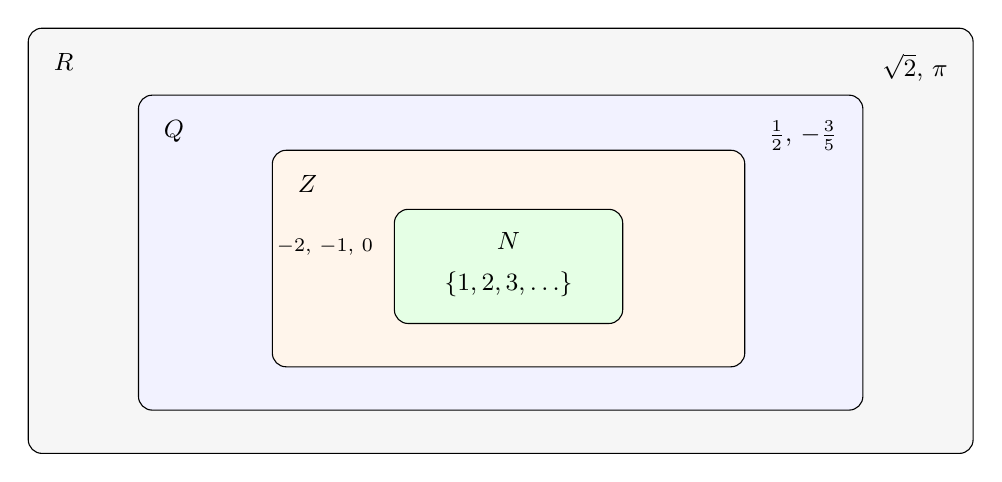
\begin{tikzpicture}[font=\small]
  \draw[rounded corners=5pt,fill=gray!7] (0,0) rectangle (12,5.4);
  \node[anchor=north west] at (0.2,5.2) {$\mathbb{R}$};
  \node[anchor=north east] at (11.8,5.2) {$\sqrt{2},\,\pi$};
  \draw[rounded corners=5pt,fill=blue!5] (1.4,0.55) rectangle (10.6,4.55);
  \node[anchor=north west] at (1.6,4.35) {$\mathbb{Q}$};
  \node[anchor=north east] at (10.4,4.35) {$\frac12,\,-\frac35$};
  \draw[rounded corners=5pt,fill=orange!8] (3.1,1.1) rectangle (9.1,3.85);
  \node[anchor=north west] at (3.3,3.65) {$\mathbb{Z}$};
  \node[anchor=north east] at (4.5,2.85) {\scriptsize $-2,\,-1,\,0$};
  \draw[rounded corners=5pt,fill=green!10] (4.65,1.65) rectangle (7.55,3.1);
  \node at (6.1,2.7) {$\mathbb{N}$};
  \node at (6.1,2.15) {$\{1,2,3,\ldots\}$};
\end{tikzpicture}

\end{figuranotas}

\section{Estructura de campo ordenado de \texorpdfstring{$\mathbb{R}$}{R}}

Los números reales poseen estructuras matemáticas importantes. La primera que estudiaremos es que $\mathbb{R}$ es un \indexemph{campo ordenado}. Esto significa que, además de satisfacer las propiedades algebraicas de un campo, sus elementos pueden compararse mediante una relación de orden compatible con la suma y el producto. Aunque esta propiedad puede parecer natural, no todos los campos pueden dotarse de un orden de este tipo. El ejemplo fundamental es el campo de los números complejos.

\begin{definition}
El conjunto de los \indexemph{números complejos} se define por
\[
\mathbb{C}=\{a+bi:a,b\in\mathbb{R}\},
\]
donde $i$ es un elemento que satisface $i^2=-1$. Si $z=a+bi\in\mathbb{C}$, llamamos \indexemph{parte real} y \indexemph{parte imaginaria} de $z$ a
\[
\operatorname{Re}(z)=a,\qquad \operatorname{Im}(z)=b.
\]
\end{definition}

\begin{example}
Son números complejos
\[
2+3i,\qquad -1+i,\qquad 4-7i,\qquad 5,\qquad -2i.
\]
Todo número real es también complejo, pues $a=a+0i$ para todo $a\in\mathbb{R}$. Por tanto,
\[
\mathbb{R}\subseteq\mathbb{C}.
\]
\end{example}

\begin{example}
El campo $\mathbb{C}$ no puede dotarse de un orden que sea compatible con sus operaciones. En efecto, en cualquier campo ordenado se cumple $x^2\geq0$ para todo $x$. Si $\mathbb{C}$ fuera un campo ordenado, entonces $i^2\geq0$; pero $i^2=-1$, por lo que tendríamos $-1\geq0$, contradiciendo que $1>0$. Por tanto, $\mathbb{C}$ no es un campo ordenado.
\end{example}

En el ejemplo anterior se anticipó una consecuencia de los axiomas de campo ordenado: el cuadrado de cualquier elemento es no negativo. Después de formalizar el orden, demostraremos esta y otras reglas que explican cómo operar con desigualdades.

\begin{definition}
Un campo $K$ se denomina \indexemph{campo ordenado} si está provisto de una relación $\leq$ que es un orden total y es compatible con las operaciones del campo. Esto significa que para cualesquiera $a,b,c\in K$ se cumplen:
\begin{enumerate}
    \item \textbf{Reflexividad:} $a\leq a$;
    \item \textbf{Antisimetría:} si $a\leq b$ y $b\leq a$, entonces $a=b$;
    \item \textbf{Transitividad:} si $a\leq b$ y $b\leq c$, entonces $a\leq c$;
    \item \textbf{Totalidad o comparabilidad:} $a\leq b$ o $b\leq a$;
    \item \textbf{Compatibilidad con la suma (invariancia por traslación):} si $a\leq b$, entonces $a+c\leq b+c$;
    \item \textbf{Compatibilidad multiplicativa (producto de no negativos):} si $0\leq a$ y $0\leq b$, entonces $0\leq ab$.
\end{enumerate}
\end{definition}

Las primeras cuatro condiciones dicen que cualquier par de elementos puede compararse en un orden coherente. Las dos últimas exigen que la comparación sea compatible con la suma y que el producto de elementos no negativos siga siendo no negativo. La notación $a<b$ significa que $a\leq b$ y $a\ne b$; equivalentemente, $a>b$ significa $b<a$.

\begin{proposition}[Comparación mediante la diferencia]
Para cualesquiera $a,b\in K$,
\[
a\leq b\quad\Longleftrightarrow\quad 0\leq b-a.
\]
En particular, $a<b$ si y sólo si $0<b-a$.
\end{proposition}

\begin{proof}
Sumar el mismo elemento preserva el orden. Por tanto, al sumar $-a$ a $a\leq b$ obtenemos $0\leq b-a$. Recíprocamente, al sumar $a$ a $0\leq b-a$ se obtiene $a\leq b$. Si alguna de las desigualdades es estricta, la otra también lo es: sumar o restar el mismo elemento no convierte dos elementos distintos en iguales.
\end{proof}

\begin{proposition}[Tricotomía]
Para cualesquiera $a,b\in K$ se cumple exactamente una de las siguientes posibilidades:
\[
a<b,\qquad a=b,\qquad b<a.
\]
\end{proposition}

\begin{proof}
Por totalidad, $a\leq b$ o $b\leq a$. Si ambas relaciones se cumplen, la antisimetría implica $a=b$. Si $a\ne b$, por tanto, sólo una de las dos comparaciones puede cumplirse y es estricta.
\end{proof}

\begin{proposition}[Positividad de $1$ y de los cuadrados]
En todo campo ordenado, $0<1$. Además, para cada $x\in K$,
\[
x^2\geq0,
\]
y si $x\ne0$, entonces $x^2>0$.
\end{proposition}

\begin{proof}
Por totalidad, $0\leq1$ o $1\leq0$. Si $1\leq0$, como $1\ne0$ tendríamos $1<0$, y al sumar $-1$ se obtendría $0<-1$. La compatibilidad del orden con el producto daría $0\leq(-1)(-1)=1$. Junto con $1\leq0$, esto implicaría $1=0$ por antisimetría, una contradicción. Así, $0\leq1$; como $1\ne0$, en realidad $0<1$.

Por tricotomía, $0\leq x$ o $x<0$. En el primer caso el axioma del producto da $x^2\geq0$. En el segundo, al sumar $-x$ a $x<0$ vemos que $0<-x$, y de nuevo el axioma del producto da $(-x)^2=x^2\geq0$. Si $x\ne0$, el producto $x^2$ no es cero por la propiedad de producto nulo; por ello $x^2>0$.
\end{proof}

Estas consecuencias justifican varias reglas prácticas: se puede sumar o restar el mismo número a ambos lados sin cambiar el sentido; multiplicar por un número positivo conserva el sentido; y multiplicar por uno negativo lo invierte. Para esta última regla es esencial conocer el signo del factor.

La relación de orden nos permite expresar comparaciones mediante desigualdades. Escribimos $a<b$ cuando $a\leq b$ y $a\neq b$; de manera análoga, $a>b$ significa $b<a$ y $a\geq b$ significa $b\leq a$. Así, por ejemplo,
\[
2<5,\qquad -3<0,\qquad 4\leq4,\qquad 7>2.
\]
También pueden escribirse desigualdades encadenadas. La expresión $a<x<b$ significa simultáneamente $a<x$ y $x<b$. Por ejemplo,
\[
1<2<5
\]
significa que $1<2$ y $2<5$. De igual manera, $a\leq x<b$ significa $a\leq x$ y $x<b$.

Las desigualdades son compatibles con las operaciones algebraicas. Si $a<b$, entonces para todo $c\in\mathbb{R}$ se cumple
\[
a+c<b+c.
\]
Por ejemplo, de $2<5$ obtenemos $2+3<5+3$, es decir, $5<8$. Si además $c>0$, entonces
\[
ac<bc,
\]
mientras que si $c<0$, el sentido de la desigualdad se invierte:
\[
ac>bc.
\]
Por ejemplo, de $2<5$ y $-3<0$ obtenemos
\[
-6>-15.
\]

\begin{proposition}[Multiplicación de desigualdades]
Sean $a,b,c\in K$ y supongamos que $a<b$. Entonces:
\begin{enumerate}
    \item si $c>0$, entonces $ac<bc$;
    \item si $c<0$, entonces $ac>bc$.
\end{enumerate}
En particular, multiplicar por $-1$ invierte la desigualdad:
\[
a<b\quad\Longrightarrow\quad -b<-a.
\]
\end{proposition}

\begin{proof}
Por la caracterización mediante la diferencia, $0<b-a$. Si $c>0$, el producto $c(b-a)$ es no negativo por el axioma del orden y no es cero por la propiedad de producto nulo. Por tanto, $0<c(b-a)=bc-ac$, de donde $ac<bc$.

Si $c<0$, al sumar $-c$ a ambos lados se obtiene $0<-c$. El mismo argumento da $0<(-c)(b-a)$. Sumando $-(-c)(b-a)$ a ambos lados de esta última desigualdad se obtiene $c(b-a)<0$. Por consiguiente, $bc-ac<0$, es decir, $bc<ac$. Para la última afirmación tomamos $c=-1$; al sumar $-1$ a $0<1$ se obtiene $-1<0$.
\end{proof}

\begin{example}
De $2<5$, al multiplicar por $-3<0$ se obtiene $-6>-15$. En cambio, al multiplicar por $3>0$ se conserva el sentido y se obtiene $6<15$. Estos dos casos muestran por qué siempre debemos revisar el signo del factor.
\end{example}

\begin{figuranotas}{Multiplicar una desigualdad por un número negativo invierte el orden.}{fig:inversion-desigualdad}
\begin{tikzpicture}[>=Stealth,font=\small]
  \node[anchor=east] at (-0.35,2) {$t$};
  \draw[->] (0,2) -- (7,2);
  \fill (2,2) circle (2pt) node[above=5pt] {$2$};
  \fill (5,2) circle (2pt) node[above=5pt] {$5$};
  \node[anchor=east] at (-0.35,0) {$-3t$};
  \draw[->] (0,0) -- (7,0);
  \fill (2,0) circle (2pt) node[below=5pt] {$-15$};
  \fill (5,0) circle (2pt) node[below=5pt] {$-6$};
  \draw[gray,dashed,->] (2,1.86) to[bend right=12] (5,0.14);
  \draw[gray,dashed,->] (5,1.86) to[bend left=12] (2,0.14);
  \node at (6.15,1) {$t\mapsto-3t$};
\end{tikzpicture}

\end{figuranotas}

\begin{proposition}[Orden de los recíprocos positivos]
Si $0<y<x$, entonces
\[
0<\frac1x<\frac1y.
\]
Así, al tomar recíprocos de dos números positivos, el orden se invierte.
\end{proposition}

\begin{proof}
Para $v\ne0$ usamos la notación $u/v:=uv^{-1}$. Primero observamos que si $t>0$, entonces $t^{-1}>0$. En efecto, $t^{-1}\ne0$. Si fuera negativo, al multiplicar $0<t$ por $t^{-1}<0$ resultaría $1=tt^{-1}<0$, en contradicción con $0<1$.

Como $x,y>0$, también $xy>0$ y, por lo anterior, $(xy)^{-1}>0$. Además, $x-y>0$. Por tanto,
\[
=\frac1y-\frac1x
=\frac{x}{xy}-\frac{y}{xy}
=\frac{x-y}{xy}
=(x-y)(xy)^{-1}>0,
\]
lo que equivale a $1/x<1/y$. La positividad de ambos recíprocos da la primera desigualdad.
\end{proof}

\begin{example}
Como $0<2<5$, sus recíprocos satisfacen
\[
0<\frac15<\frac12.
\]
La hipótesis de positividad importa: no se puede tomar recíprocos de una desigualdad que atraviesa el cero, y el orden debe analizarse por separado cuando los números son negativos.
\end{example}

Las desigualdades permiten describir de forma natural ciertos subconjuntos fundamentales de $\mathbb{R}$ llamados intervalos.

\begin{definition}
Sean $a,b\in\mathbb{R}$ con $a<b$. Definimos los \indexemph{intervalos acotados} por
\begin{enumerate}
    \item
    \[
    (a,b)=\{x\in\mathbb{R}:a<x<b\};
    \]

    \item
    \[
    [a,b)=\{x\in\mathbb{R}:a\leq x<b\};
    \]

    \item
    \[
    (a,b]=\{x\in\mathbb{R}:a<x\leq b\};
    \]

    \item
    \[
    [a,b]=\{x\in\mathbb{R}:a\leq x\leq b\}.
    \]
\end{enumerate}
El intervalo $(a,b)$ se denomina \indexemph{abierto}, $[a,b]$ se denomina \indexemph{cerrado}, mientras que $[a,b)$ y $(a,b]$ se denominan \indexemph{semiabiertos} o \indexemph{semicerrados}.
\end{definition}

\begin{example}
El intervalo
\[
(1,4)=\{x\in\mathbb{R}:1<x<4\}
\]
contiene, por ejemplo, a $2$, $3$ y $\pi$, pero no contiene a $1$ ni a $4$.
\end{example}

\begin{example}
El intervalo
\[
[1,4)=\{x\in\mathbb{R}:1\leq x<4\}
\]
contiene a $1$ pero no contiene a $4$, mientras que
\[
(1,4]
\]
contiene a $4$ pero no a $1$. Finalmente,
\[
[1,4]
\]
contiene ambos extremos.
\end{example}

\begin{figuranotas}{Intervalos acotados y pertenencia de sus extremos.}{fig:intervalos-acotados}
\begin{tikzpicture}[>=Stealth,font=\small]
  % Intervalo abierto: los dos extremos quedan fuera.
  \node[anchor=east] at (1.15,3) {$(a,b)$};
  \draw[<->,gray] (1.4,3) -- (6.8,3);
  \draw[very thick,blue!65] (2.4,3) -- (5.8,3);
  \draw[draw=blue!65,fill=white,thick] (2.4,3) circle (2.3pt);
  \draw[draw=blue!65,fill=white,thick] (5.8,3) circle (2.3pt);
  \node[below=4pt] at (2.4,3) {$a$};
  \node[below=4pt] at (5.8,3) {$b$};

  % Intervalo cerrado: los dos extremos se incluyen.
  \node[anchor=east] at (1.15,2) {$[a,b]$};
  \draw[<->,gray] (1.4,2) -- (6.8,2);
  \draw[very thick,blue!65] (2.4,2) -- (5.8,2);
  \fill[blue!65] (2.4,2) circle (2.3pt);
  \fill[blue!65] (5.8,2) circle (2.3pt);
  \node[below=4pt] at (2.4,2) {$a$};
  \node[below=4pt] at (5.8,2) {$b$};

  % Intervalos semiabiertos: se incluye exactamente uno de los extremos.
  \node[anchor=east] at (1.15,1) {$[a,b)$};
  \draw[<->,gray] (1.4,1) -- (6.8,1);
  \draw[very thick,blue!65] (2.4,1) -- (5.8,1);
  \fill[blue!65] (2.4,1) circle (2.3pt);
  \draw[draw=blue!65,fill=white,thick] (5.8,1) circle (2.3pt);
  \node[below=4pt] at (2.4,1) {$a$};
  \node[below=4pt] at (5.8,1) {$b$};

  \node[anchor=east] at (1.15,0) {$(a,b]$};
  \draw[<->,gray] (1.4,0) -- (6.8,0);
  \draw[very thick,blue!65] (2.4,0) -- (5.8,0);
  \draw[draw=blue!65,fill=white,thick] (2.4,0) circle (2.3pt);
  \fill[blue!65] (5.8,0) circle (2.3pt);
  \node[below=4pt] at (2.4,0) {$a$};
  \node[below=4pt] at (5.8,0) {$b$};
\end{tikzpicture}

\end{figuranotas}
En estas gráficas, el círculo vacío indica que el extremo no pertenece al intervalo y el punto lleno indica que sí pertenece.

También necesitamos describir conjuntos que se extienden indefinidamente hacia alguno de los dos sentidos de la recta real. Para ello utilizamos los símbolos $\infty$ y $-\infty$. Estos símbolos no representan números reales y, por tanto,
\[
\infty\notin\mathbb{R},\qquad -\infty\notin\mathbb{R}.
\]
Su función es únicamente indicar que un intervalo no posee un extremo real en cierta dirección.

\begin{definition}
Sea $a\in\mathbb{R}$. Los \indexemph{intervalos no acotados} se definen por
\[
(a,\infty)=\{x\in\mathbb{R}:a<x\},\qquad [a,\infty)=\{x\in\mathbb{R}:a\leq x\},
\]
y
\[
(-\infty,a)=\{x\in\mathbb{R}:x<a\},\qquad (-\infty,a]=\{x\in\mathbb{R}:x\leq a\}.
\]
Además,
\[
\mathbb{R}=(-\infty,\infty).
\]
\end{definition}

\begin{example}
El intervalo
\[
(2,\infty)=\{x\in\mathbb{R}:x>2\}
\]
contiene a $3$, $\pi$ y $10$, pero no contiene a $2$.
\end{example}

\begin{example}
El intervalo
\[
[2,\infty)=\{x\in\mathbb{R}:x\geq2\}
\]
contiene a $2$ y a todos los números reales mayores que él.
\end{example}

\begin{example}
El intervalo
\[
(-\infty,3)=\{x\in\mathbb{R}:x<3\}
\]
contiene, por ejemplo, a $-5$, $0$ y $\sqrt2$, pero no contiene a $3$.
\end{example}

\begin{example}
El intervalo
\[
(-\infty,3]=\{x\in\mathbb{R}:x\leq3\}
\]
contiene a todos los números reales menores o iguales que $3$, incluido el propio $3$.
\end{example}

\begin{figuranotas}{Intervalos no acotados: los extremos infinitos indican una dirección, no un punto.}{fig:intervalos-no-acotados}
\begin{tikzpicture}[>=Stealth,font=\small]
  \node[anchor=east] at (1.15,3) {$(a,\infty)$};
  \draw[very thick,blue!65,->] (3.4,3) -- (7.1,3);
  \draw[fill=white,blue!65,thick] (3.4,3) circle (2.3pt);
  \node[below=4pt] at (3.4,3) {$a$};

  \node[anchor=east] at (1.15,2) {$[a,\infty)$};
  \draw[very thick,blue!65,->] (3.4,2) -- (7.1,2);
  \fill[blue!65] (3.4,2) circle (2.3pt);
  \node[below=4pt] at (3.4,2) {$a$};

  \node[anchor=east] at (1.15,1) {$(-\infty,a)$};
  \draw[very thick,blue!65,<-] (1.4,1) -- (3.4,1);
  \draw[fill=white,blue!65,thick] (3.4,1) circle (2.3pt);
  \node[below=4pt] at (3.4,1) {$a$};

  \node[anchor=east] at (1.15,0) {$(-\infty,a]$};
  \draw[very thick,blue!65,<-] (1.4,0) -- (3.4,0);
  \fill[blue!65] (3.4,0) circle (2.3pt);
  \node[below=4pt] at (3.4,0) {$a$};

  \node[anchor=east] at (1.15,-1) {$\mathbb{R}$};
  \draw[very thick,blue!65,<->] (1.4,-1) -- (7.1,-1);
\end{tikzpicture}

\end{figuranotas}
Las flechas muestran que el intervalo continúa indefinidamente en esa dirección; no señalan un extremo real llamado $\infty$ o $-\infty$.

Enseguida verificamos que el orden usual de los números reales es compatible con su estructura algebraica.

\begin{proposition}
El campo $\mathbb{R}$, provisto de su orden usual $\leq$, es un campo ordenado.
\end{proposition}

\begin{proof}
La relación $\leq$ en $\mathbb{R}$ es reflexiva, antisimétrica, transitiva y total. Además, para cualesquiera $a,b,c\in\mathbb{R}$, si $a\leq b$, entonces $a+c\leq b+c$, y si $0\leq a$ y $0\leq b$, entonces $0\leq ab$. Por tanto, el orden usual de $\mathbb{R}$ es compatible con las operaciones de suma y producto, y en consecuencia $\mathbb{R}$ es un campo ordenado.
\end{proof}

\section{Valor absoluto y desigualdades}
Una parte importante del análisis real se fundamenta en el estudio de desigualdades. Estas permiten comparar cantidades, obtener estimaciones y controlar el comportamiento de expresiones que posteriormente aparecerán en sucesiones, límites, continuidad y convergencia. Una de las herramientas más elementales y, al mismo tiempo, más utilizadas para expresar este tipo de estimaciones es el valor absoluto.

\begin{definition}[Valor absoluto]
Sea $x\in\mathbb{R}$. El \indexemph{valor absoluto} de $x$ se define por
\[
|x|=
\begin{cases}
x, & x\geq0,\\
-x, & x<0.
\end{cases}
\]
En particular, $|x|\geq0$ para todo $x\in\mathbb{R}$ y $|x|=0$ si y sólo si $x=0$.
\end{definition}

\begin{proposition}[Relación entre el valor absoluto y el cuadrado]
Para todo $x\in\mathbb{R}$,
\[
(|x|)^2=x^2,
\qquad
|x^2|=x^2,
\qquad\text{y, por consiguiente,}\qquad
|x|=\sqrt{x^2}.
\]
\end{proposition}

\begin{proof}
Si $x\geq0$, entonces $|x|=x$, así que $(|x|)^2=x^2$. Si $x<0$, entonces $|x|=-x$ y de nuevo $(|x|)^2=(-x)^2=x^2$. En ambos casos $x^2\geq0$, por lo que $|x^2|=x^2$. Además, $|x|$ es no negativo y su cuadrado es $x^2$; por la unicidad de la raíz cuadrada no negativa, $|x|=\sqrt{x^2}$.
\end{proof}

\begin{example}
Por definición,
\[
|5|=5,\qquad |-5|=5,\qquad |0|=0.
\]
El valor absoluto puede interpretarse como la distancia de un número al origen; por ello, tanto $5$ como $-5$ se encuentran a distancia $5$ de $0$.
\end{example}

\begin{example}
Si $x=-3$, entonces $|x|=3$. Además,
\[
-|x|\leq x\leq |x|,
\]
pues en este caso
\[
-3\leq -3\leq3.
\]
En general, esta desigualdad se cumple para todo $x\in\mathbb{R}$.
\end{example}

\begin{proposition}[Cotas inmediatas del valor absoluto]
Para todo $x\in\mathbb{R}$,
\[
-|x|\leq x\leq |x|.
\]
\end{proposition}

\begin{proof}
Si $x\geq0$, entonces $|x|=x$ y $-|x|=-x\leq x$. Si $x<0$, entonces $|x|=-x$ y $-|x|=x\leq -x=|x|$. En ambos casos la afirmación sigue de la definición por casos del valor absoluto y del orden usual.
\end{proof}

El valor absoluto también permite expresar desigualdades de una manera especialmente compacta. Si $r>0$, entonces
\[
|x|<r
\]
significa que la distancia de $x$ al origen es menor que $r$, lo cual equivale a
\[
-r<x<r.
\]
De manera análoga,
\[
|x|\leq r\quad\Longleftrightarrow\quad -r\leq x\leq r.
\]
Estas equivalencias se leen directamente de la definición: si $x\geq0$, entonces $|x|=x$; si $x<0$, entonces $|x|=-x$. En ambos casos, comparar $|x|$ con $r>0$ equivale a exigir que $x$ no quede ni a la izquierda de $-r$ ni a la derecha de $r$.
Esta observación permite describir intervalos centrados en cualquier punto de la recta real.

\begin{proposition}
Sean $a,x\in\mathbb{R}$ y $r>0$. Entonces
\[
x\in(a-r,a+r)
\quad\Longleftrightarrow\quad
|x-a|<r.
\]
De manera análoga,
\[
x\in[a-r,a+r]
\quad\Longleftrightarrow\quad
|x-a|\leq r.
\]
\end{proposition}

\begin{proof}
Por definición,
\[
x\in(a-r,a+r)
\]
si y sólo si
\[
a-r<x<a+r.
\]
Restando $a$ en los tres miembros obtenemos
\[
-r<x-a<r.
\]
Por la caracterización del valor absoluto,
\[
-r<x-a<r
\quad\Longleftrightarrow\quad
|x-a|<r.
\]
Por tanto,
\[
x\in(a-r,a+r)
\quad\Longleftrightarrow\quad
|x-a|<r.
\]
El caso cerrado se demuestra de manera análoga utilizando desigualdades no estrictas.
En efecto,
\[
x\in[a-r,a+r]
\quad\Longleftrightarrow\quad
a-r\leq x\leq a+r
\quad\Longleftrightarrow\quad
-r\leq x-a\leq r
\quad\Longleftrightarrow\quad
|x-a|\leq r.
\]
\end{proof}

La equivalencia de esta proposición también tiene una lectura geométrica: $|x-a|<r$ describe los puntos cuya distancia a $a$ es menor que $r$. En la recta real son exactamente los puntos del intervalo abierto con centro $a$ y radio $r$.

\begin{figuranotas}{El valor absoluto como distancia a un centro.}{fig:valor-absoluto-intervalo}
\begin{tikzpicture}[>=Stealth,font=\small]
  \draw[->] (0,0) -- (10,0) node[right] {$\mathbb{R}$};
  \draw[very thick,blue!65] (2.5,0) -- (7.5,0);
  \draw[blue!65,thick] (2.5,-0.13) -- (2.5,0.13);
  \draw[blue!65,thick] (7.5,-0.13) -- (7.5,0.13);
  \draw[fill=white,thick] (2.5,0) circle (2.2pt);
  \draw[fill=white,thick] (7.5,0) circle (2.2pt);
  \fill (5,0) circle (2pt);
  \fill (4.25,0) circle (2pt);
  \node[above=5pt] at (2.5,0.13) {$a-r$};
  \node[above=5pt] at (7.5,0.13) {$a+r$};
  \node[above=5pt] at (5,0.04) {$a$};
  \node[below=5pt] at (4.25,-0.02) {$x$};
  \draw[<->] (2.5,-0.72) -- (5,-0.72);
  \node[below=3pt] at (3.75,-0.72) {$r$};
  \node[below=3pt] at (6.0,-1.0) {$|x-a|<r\;\Longleftrightarrow\;a-r<x<a+r$};
\end{tikzpicture}

\end{figuranotas}

\begin{example}
La desigualdad
\[
|x-3|<2
\]
equivale a
\[
-2<x-3<2,
\]
y sumando $3$ obtenemos
\[
1<x<5.
\]
Por tanto,
\[
|x-3|<2
\quad\Longleftrightarrow\quad
x\in(1,5).
\]
\end{example}

Otra propiedad fundamental es que el valor absoluto es compatible con el producto.

\begin{proposition}
Para cualesquiera $x,y\in\mathbb{R}$ se cumple
\[
|xy|=|x||y|.
\]
\end{proposition}

\begin{proof}
Como $|x|^2=x^2$ y $|y|^2=y^2$, tenemos
\[
|xy|^2=x^2y^2=|x|^2|y|^2=(|x||y|)^2.
\]
Puesto que $|xy|\geq0$ y $|x||y|\geq0$, la igualdad de sus cuadrados implica que son iguales. En efecto, si $u,v\geq0$ y $u^2=v^2$, entonces $(u-v)(u+v)=0$; si $u+v=0$, ambos son cero, y si $u+v>0$, necesariamente $u-v=0$. Se sigue que
\[
|xy|=|x||y|.
\]
\end{proof}

Una de las desigualdades fundamentales del análisis es la \indexemph{desigualdad del triángulo}. Su nombre proviene de su interpretación geométrica: la longitud de uno de los lados de un triángulo nunca puede superar la suma de las longitudes de los otros dos. En la recta real, esta propiedad se expresa mediante valores absolutos.

\begin{proposition}[Desigualdad del triángulo]
Para cualesquiera $x,y\in\mathbb{R}$ se cumple
\[
|x+y|\leq |x|+|y|.
\]
\end{proposition}

\begin{proof}
Como
\[
xy\leq |x||y|,
\]
tenemos
\[
(x+y)^2=x^2+2xy+y^2
\leq x^2+2|x||y|+y^2
=(|x|+|y|)^2.
\]
Además, tanto $|x+y|$ como $|x|+|y|$ son no negativos. Tomando raíces cuadradas obtenemos
\[
|x+y|\leq|x|+|y|.
\]
\end{proof}

La desigualdad del triángulo posee una forma inversa que será utilizada reiteradamente para comparar distancias.

\begin{proposition}[Desigualdad triangular inversa]
Para cualesquiera $x,y\in\mathbb{R}$ se cumple
\[
|x-y|\geq \bigl||x|-|y|\bigr|.
\]
\end{proposition}

\begin{proof}
Por la desigualdad del triángulo,
\[
|x|=|(x-y)+y|\leq|x-y|+|y|,
\]
de donde
\[
|x|-|y|\leq|x-y|.
\]
Intercambiando $x$ e $y$ obtenemos
\[
|y|-|x|\leq|x-y|.
\]
Por tanto,
\[
-\lvert x-y\rvert\leq |x|-|y|\leq|x-y|,
\]
y, por la caracterización del valor absoluto,
\[
\bigl||x|-|y|\bigr|\leq|x-y|.
\]
\end{proof}

\begin{example}
Si $x=3$ y $y=-5$, entonces la desigualdad del triángulo establece
\[
|3+(-5)|\leq|3|+|-5|,
\]
es decir,
\[
2\leq8.
\]
\end{example}

\begin{example}
Para $x=-4$ y $y=7$ tenemos
\[
|x-y|=|-11|=11,
\]
mientras que
\[
\bigl||x|-|y|\bigr|=|4-7|=3.
\]
Por tanto,
\[
11\geq3,
\]
como establece la desigualdad triangular inversa.
\end{example}

\begin{example}
La desigualdad
\[
|x-5|\leq3
\]
equivale a
\[
-3\leq x-5\leq3.
\]
Sumando $5$ obtenemos
\[
2\leq x\leq8,
\]
por lo que
\[
|x-5|\leq3
\quad\Longleftrightarrow\quad
x\in[2,8].
\]
\end{example}

\begin{example}
Sean $x,y,z\in\mathbb{R}$. Aplicando dos veces la desigualdad del triángulo obtenemos
\[
|x+y+z|\leq |x+y|+|z|
\leq |x|+|y|+|z|.
\]
Esta propiedad puede extenderse inductivamente a cualquier número finito de sumandos.
\end{example}

\begin{proposition}[Desigualdad triangular finita]
Para cualesquiera $x_1,\ldots,x_n\in\mathbb{R}$ se cumple
\[
\left|\sum_{k=1}^{n}x_k\right|
\leq
\sum_{k=1}^{n}|x_k|.
\]
\end{proposition}

\begin{proof}
La demostración se realiza por inducción sobre $n$. Para $n=1$ la igualdad es inmediata. Supongamos que el resultado es válido para $n$. Entonces, por la desigualdad del triángulo,
\[
\left|\sum_{k=1}^{n+1}x_k\right|
=
\left|\sum_{k=1}^{n}x_k+x_{n+1}\right|
\leq
\left|\sum_{k=1}^{n}x_k\right|+|x_{n+1}|.
\]
Aplicando la hipótesis de inducción,
\[
\left|\sum_{k=1}^{n+1}x_k\right|
\leq
\sum_{k=1}^{n}|x_k|+|x_{n+1}|
=
\sum_{k=1}^{n+1}|x_k|.
\]
\end{proof}

Además de las desigualdades asociadas al valor absoluto, existen algunas desigualdades algebraicas elementales que aparecerán continuamente en análisis. Una de las más sencillas surge directamente del hecho de que el cuadrado de todo número real es no negativo.

\begin{proposition}
Para cualesquiera $a,b\in\mathbb{R}$ se cumple
\[
ab\leq\frac{a^2+b^2}{2}.
\]
\end{proposition}

\begin{proof}
Como
\[
(a-b)^2\geq0,
\]
se tiene
\[
a^2-2ab+b^2\geq0.
\]
Por tanto,
\[
2ab\leq a^2+b^2,
\]
y dividiendo entre $2$ obtenemos
\[
ab\leq\frac{a^2+b^2}{2}.
\]
\end{proof}

Una consecuencia inmediata es otra estimación que será útil con frecuencia.

\begin{proposition}
Para cualesquiera $a,b\in\mathbb{R}$ se cumple
\[
(a+b)^2\leq2(a^2+b^2).
\]
\end{proposition}

\begin{proof}
Tenemos
\[
(a+b)^2=a^2+2ab+b^2.
\]
Como $2ab\leq a^2+b^2$, resulta
\[
(a+b)^2
\leq
a^2+(a^2+b^2)+b^2
=
2(a^2+b^2).
\]
\end{proof}

Otra desigualdad fundamental compara la media geométrica con la media aritmética.

\begin{proposition}[Desigualdad aritmético--geométrica]
Si $a,b\geq0$, entonces
\[
\sqrt{ab}\leq\frac{a+b}{2}.
\]
La igualdad ocurre si y sólo si $a=b$.
\end{proposition}

\begin{proof}
Como
\[
(\sqrt{a}-\sqrt{b})^2\geq0,
\]
tenemos
\[
a-2\sqrt{ab}+b\geq0.
\]
Por tanto,
\[
2\sqrt{ab}\leq a+b,
\]
y dividiendo entre $2$ obtenemos
\[
\sqrt{ab}\leq\frac{a+b}{2}.
\]
La igualdad ocurre precisamente cuando
\[
(\sqrt{a}-\sqrt{b})^2=0,
\]
es decir, cuando $a=b$.
\end{proof}

Esta desigualdad forma parte de una relación más amplia entre distintas medias.

\begin{proposition}[Desigualdad de las medias]
Si $a,b>0$, entonces
\[
\frac{2ab}{a+b}
\leq
\sqrt{ab}
\leq
\frac{a+b}{2}
\leq
\sqrt{\frac{a^2+b^2}{2}}.
\]
\end{proposition}

\begin{proof}
La desigualdad central ya fue demostrada. Probemos con detalle la primera comparación. Como $a,b>0$, también $a+b>0$ y $\sqrt{ab}>0$. Partimos de
\[
2\sqrt{ab}\leq a+b
\]
y multiplicamos ambos lados por $\sqrt{ab}/(a+b)>0$. Al simplificar,
\[
\frac{2ab}{a+b}\leq\sqrt{ab}.
\]
Así queda justificado que la desigualdad conserva su sentido: el factor por el que multiplicamos es positivo.

Por otra parte,
\[
(a+b)^2\leq2(a^2+b^2),
\]
por lo que
\[
\frac{(a+b)^2}{4}\leq\frac{a^2+b^2}{2}.
\]
Tomando raíces cuadradas,
\[
\frac{a+b}{2}\leq\sqrt{\frac{a^2+b^2}{2}}.
\]
En la comparación armónica--geométrica, la transformación anterior sólo multiplica por un factor positivo, así que la igualdad equivale a $2\sqrt{ab}=a+b$. En la comparación geométrica--aritmética, la igualdad ocurre cuando $(\sqrt a-\sqrt b)^2=0$. Ambas condiciones equivalen a $a=b$. En la comparación aritmética--cuadrática, la igualdad equivale a $(a-b)^2=0$, por lo que también requiere $a=b$. Por tanto, las cuatro medias coinciden exactamente cuando $a=b$.
\end{proof}

\begin{example}
Para $a=1$ y $b=4$, las medias armónica, geométrica, aritmética y cuadrática son, respectivamente,
\[
\frac{2\cdot1\cdot4}{1+4}=\frac85,
\qquad
\sqrt{1\cdot4}=2,
\qquad
\frac{1+4}{2}=\frac52,
\qquad
\sqrt{\frac{1^2+4^2}{2}}=\sqrt{\frac{17}{2}}.
\]
En efecto,
\[
1.6\leq2\leq2.5\leq\sqrt{8.5}.
\]
\end{example}

\begin{figuranotas}{Las cuatro medias del ejemplo ordenadas sobre la recta real: $H$ es la armónica, $G$ la geométrica, $A$ la aritmética y $Q$ la cuadrática.}{fig:orden-medias}
\begin{tikzpicture}[>=Stealth,font=\small]
  \draw[->] (0,0) -- (10,0);
  \foreach \x/\val/\pos/\mean in {
    2/{\frac85}/above/H,
    4/{2}/above/G,
    6.5/{\frac52}/above/A,
    8.58/{\sqrt{17/2}}/above/Q
  } {
    \fill[blue!65] (\x,0) circle (2pt);
    \node[\pos=5pt] at (\x,0) {$\val$};
    \node[below=5pt] at (\x,0) {$\mean$};
  }
  \node[below=23pt] at (5,0) {$H\leq G\leq A\leq Q$};
\end{tikzpicture}

\end{figuranotas}

Otra desigualdad elemental de gran utilidad es la \indexemph{desigualdad de Bernoulli}, que permite estimar potencias sin necesidad de desarrollarlas completamente.

\begin{proposition}[Desigualdad de Bernoulli]
Sea $a\geq-1$ y $n\in\mathbb{N}$. Entonces
\[
(1+a)^n\geq1+na.
\]
\end{proposition}

\begin{proof}
Procedemos por inducción sobre $n$. Para $n=1$,
\[
(1+a)^1=1+a,
\]
por lo que el resultado es cierto. Supongamos ahora que
\[
(1+a)^n\geq1+na.
\]
Como $a\geq-1$, tenemos $1+a\geq0$ y podemos multiplicar la desigualdad por $1+a$:
\[
(1+a)^{n+1}\geq(1+na)(1+a).
\]
Desarrollando,
\[
(1+na)(1+a)
=
1+(n+1)a+na^2.
\]
Como $na^2\geq0$,
\[
(1+a)^{n+1}\geq1+(n+1)a.
\]
Por el principio de inducción matemática, la desigualdad se cumple para todo $n\in\mathbb{N}$.
\end{proof}

\begin{example}
Tomando $a=0.1$ y $n=5$, la desigualdad de Bernoulli proporciona
\[
(1.1)^5\geq1+5(0.1)=1.5.
\]
En efecto,
\[
(1.1)^5=1.61051\geq1.5.
\]
\end{example}

Una de las desigualdades más importantes de las matemáticas es la \indexemph{desigualdad de Cauchy--Schwarz}. En el caso finito puede formularse exclusivamente en términos de números reales.

\begin{proposition}[Desigualdad de Cauchy--Schwarz]
Sean $a_1,\ldots,a_n,b_1,\ldots,b_n\in\mathbb{R}$. Entonces
\[
\left(\sum_{k=1}^{n}a_kb_k\right)^2
\leq
\left(\sum_{k=1}^{n}a_k^2\right)
\left(\sum_{k=1}^{n}b_k^2\right).
\]
\end{proposition}

\begin{proof}
Si
\[
\sum_{k=1}^{n}b_k^2=0,
\]
entonces $b_k=0$ para todo $k$ y la desigualdad es inmediata. Supongamos, por tanto, que
\[
\sum_{k=1}^{n}b_k^2>0
\]
y definamos
\[
\lambda=
\frac{\displaystyle\sum_{k=1}^{n}a_kb_k}
{\displaystyle\sum_{k=1}^{n}b_k^2}.
\]
Como todo cuadrado es no negativo,
\[
0\leq\sum_{k=1}^{n}(a_k-\lambda b_k)^2.
\]
Desarrollando y sustituyendo el valor de $\lambda$ obtenemos
\[
0\leq
\sum_{k=1}^{n}a_k^2
-
\frac{\left(\sum_{k=1}^{n}a_kb_k\right)^2}
{\sum_{k=1}^{n}b_k^2}.
\]
Multiplicando por $\sum_{k=1}^{n}b_k^2>0$ resulta
\[
\left(\sum_{k=1}^{n}a_kb_k\right)^2
\leq
\left(\sum_{k=1}^{n}a_k^2\right)
\left(\sum_{k=1}^{n}b_k^2\right).
\]
\end{proof}

\begin{example}
Para $(a_1,a_2)=(1,2)$ y $(b_1,b_2)=(3,4)$, Cauchy--Schwarz establece
\[
(1\cdot3+2\cdot4)^2
\leq
(1^2+2^2)(3^2+4^2).
\]
En efecto,
\[
121\leq125.
\]
\end{example}

Como consecuencia de Cauchy--Schwarz obtenemos una desigualdad útil para sumas.

\begin{proposition}
Para cualesquiera $x_1,\ldots,x_n\in\mathbb{R}$ se cumple
\[
\left(\sum_{k=1}^{n}x_k\right)^2
\leq
n\sum_{k=1}^{n}x_k^2.
\]
\end{proposition}

\begin{proof}
Aplicando Cauchy--Schwarz a los números
\[
a_k=x_k,
\qquad
b_k=1,
\]
obtenemos
\[
\left(\sum_{k=1}^{n}x_k\right)^2
\leq
\left(\sum_{k=1}^{n}x_k^2\right)
\left(\sum_{k=1}^{n}1^2\right).
\]
Como
\[
\sum_{k=1}^{n}1^2=n,
\]
se concluye que
\[
\left(\sum_{k=1}^{n}x_k\right)^2
\leq
n\sum_{k=1}^{n}x_k^2.
\]
\end{proof}

Estas desigualdades constituyen herramientas elementales que aparecerán reiteradamente a lo largo del análisis. En particular, el valor absoluto y la desigualdad del triángulo permitirán formalizar la noción de distancia, mientras que Bernoulli, las desigualdades entre medias y Cauchy--Schwarz proporcionarán estimaciones fundamentales para el estudio posterior de sucesiones, límites y convergencia.

\section{Conjuntos acotados}
En esta sección estudiaremos qué significa que un conjunto de números reales esté limitado por arriba o por abajo y qué operaciones conservan esas propiedades. Los conjuntos acotados aparecen una y otra vez porque nos permiten controlar los valores que puede tomar un conjunto. Esta idea será importante más adelante: en el capítulo sobre sucesiones será una hipótesis central en el teorema de Bolzano--Weierstrass, y en el capítulo de topología aparecerá junto con la cerradura en el teorema de Heine--Borel. Aquí construiremos primero el lenguaje y las propiedades elementales que necesitaremos para entender esos resultados posteriores.

\begin{definition}[Cotas superiores]
Sea $A\subseteq\mathbb{R}$. Un número $M\in\mathbb{R}$ se llama \indexemph{cota superior} de $A$ si
\[
 x\leq M\qquad\text{para todo }x\in A.
\]
El \indexemph{conjunto de cotas superiores} de $A$ se denota por
\[
 U(A)=\{M\in\mathbb{R}: x\leq M\text{ para todo }x\in A\}.
\]
Decimos que $A$ está \indexemph{acotado superiormente} cuando $U(A)\neq\varnothing$.
\end{definition}

\begin{definition}[Cotas inferiores]
Sea $A\subseteq\mathbb{R}$. Un número $m\in\mathbb{R}$ se llama \indexemph{cota inferior} de $A$ si
\[
 m\leq x\qquad\text{para todo }x\in A.
\]
El \indexemph{conjunto de cotas inferiores} de $A$ se denota por
\[
 L(A)=\{m\in\mathbb{R}: m\leq x\text{ para todo }x\in A\}.
\]
Decimos que $A$ está \indexemph{acotado inferiormente} cuando $L(A)\neq\varnothing$.
\end{definition}

\begin{remark}
Para $A=\varnothing$, las condiciones que definen una cota se cumplen vacíamente para todo real. Por tanto,
\[
 U(\varnothing)=L(\varnothing)=\mathbb{R}.
\]
Así, el conjunto vacío está acotado superior e inferiormente. Sin embargo, la afirmación de que toda cota inferior está por debajo de toda cota superior requiere que $A$ no sea vacío.
\end{remark}

\begin{proposition}[Relación entre cotas inferiores y superiores]
Si $A\neq\varnothing$, $m\in L(A)$ y $M\in U(A)$, entonces $m\leq M$. Es decir, toda cota inferior de $A$ queda a la izquierda de toda cota superior.
\end{proposition}

\begin{proof}
Como $A$ no es vacío, existe $x\in A$. Por las definiciones de cota inferior y superior,
\[
 m\leq x\leq M,
\]
de donde se obtiene $m\leq M$ por transitividad. La hipótesis de que $A$ no sea vacío es necesaria: para $A=\varnothing$, los números $1\in L(A)$ y $0\in U(A)$ satisfacen $1\not\leq0$.
\end{proof}

\begin{example}
Sea $A=(0,1)$. Entonces
\[
 U(A)=[1,\infty),\qquad L(A)=(-\infty,0].
\]
En efecto, todo $M\geq1$ es mayor que cada elemento de $A$. Si $M<1$, cuando $M<0$ podemos tomar $x=1/2$, y cuando $0\leq M<1$ podemos tomar $x=(M+1)/2$; en ambos casos $x\in A$ y $x>M$, por lo que $M$ no es cota superior. Para las cotas inferiores, todo $m\leq0$ sirve. Si $m>0$, cuando $m<2$ tomamos $x=m/2$, y cuando $m\geq2$ tomamos $x=1/2$; en ambos casos $x\in A$ y $x<m$, así que $m$ no es cota inferior.
\end{example}

\begin{figuranotas}{El intervalo $A=(0,1)$ y sus conjuntos de cotas inferiores y superiores.}{fig:cotas-intervalo-abierto}
\begin{tikzpicture}[>=Stealth,font=\small]
  % A=(0,1): los puntos 0 y 1 no pertenecen al conjunto.
  \node[anchor=east] at (0.45,2) {$A=(0,1)$};
  \draw[<->,gray] (0.8,2) -- (6.8,2);
  \draw[very thick,blue!65] (2.2,2) -- (4.8,2);
  \draw[draw=blue!65,fill=white,thick] (2.2,2) circle (2.4pt);
  \draw[draw=blue!65,fill=white,thick] (4.8,2) circle (2.4pt);
  \node[below=4pt] at (2.2,2) {$0$};
  \node[below=4pt] at (4.8,2) {$1$};

  % Las cotas superiores comienzan en 1 e incluyen ese extremo.
  \node[anchor=east] at (0.45,1) {$U(A)$};
  \draw[<->,gray] (0.8,1) -- (6.8,1);
  \draw[very thick,teal!70!black,->] (4.8,1) -- (6.65,1);
  \fill[teal!70!black] (4.8,1) circle (2.4pt);
  \node[below=4pt] at (4.8,1) {$1$};

  % Las cotas inferiores terminan en 0 e incluyen ese extremo.
  \node[anchor=east] at (0.45,0) {$L(A)$};
  \draw[<->,gray] (0.8,0) -- (6.8,0);
  \draw[very thick,orange!85!black,<-] (2.2,0) -- (0.95,0);
  \fill[orange!85!black] (2.2,0) circle (2.4pt);
  \node[below=4pt] at (2.2,0) {$0$};
\end{tikzpicture}

\end{figuranotas}

\begin{example}
Para el conjunto finito $B=\{2,5,7\}$ se tiene
\[
 U(B)=[7,\infty),\qquad L(B)=(-\infty,2].
\]
Por ejemplo, $9$ es una cota superior y $1$ es una cota inferior; en cambio, $6$ no es cota superior porque $7\in B$ y $6<7$.
\end{example}

\begin{example}
El conjunto $\mathbb{R}$ no está acotado superior ni inferiormente. Dado cualquier $M\in\mathbb{R}$, el número $M+1$ pertenece a $\mathbb{R}$ y es mayor que $M$; por tanto, $M$ no es una cota superior. Análogamente, para cada $m\in\mathbb{R}$, el número $m-1$ es menor que $m$, así que $m$ no es una cota inferior. En consecuencia,
\[
 U(\mathbb{R})=L(\mathbb{R})=\varnothing.
\]
\end{example}

\begin{proposition}[Monotonía respecto de la inclusión]
Si $A\subseteq B\subseteq\mathbb{R}$, entonces
\[
 U(B)\subseteq U(A),\qquad L(B)\subseteq L(A).
\]
En particular, si $B$ está acotado superiormente (o inferiormente), todo subconjunto $A$ de $B$ también lo está.
\end{proposition}

\begin{proof}
Si $M\in U(B)$, entonces $x\leq M$ para todo $x\in B$, y en particular para todo $x\in A$; así, $M\in U(A)$. La inclusión de conjuntos de cotas inferiores se demuestra de la misma manera.
\end{proof}

\begin{proposition}[Cierre de los conjuntos de cotas]
Sea $A\subseteq\mathbb{R}$.
\begin{enumerate}
  \item Si $M\in U(A)$ y $N\geq M$, entonces $N\in U(A)$.
  \item Si $m\in L(A)$ y $n\leq m$, entonces $n\in L(A)$.
\end{enumerate}
Así, una vez que se encuentra una cota superior, todo número mayor también es cota superior; y todo número menor que una cota inferior también es cota inferior.
\end{proposition}

\begin{proof}
Si $M\in U(A)$, entonces $x\leq M$ para todo $x\in A$. De $M\leq N$ y la transitividad del orden se sigue $x\leq N$, luego $N\in U(A)$. El segundo inciso se demuestra del mismo modo: $n\leq m\leq x$ para todo $x\in A$, así que $n\in L(A)$.
\end{proof}

\begin{proposition}[Acotación superior e inferior mediante intervalos]
Un conjunto $A\subseteq\mathbb{R}$ está acotado superiormente si y solo si existe $M\in\mathbb{R}$ tal que
\[
 A\subseteq(-\infty,M].
\]
Análogamente, $A$ está acotado inferiormente si y solo si existe $m\in\mathbb{R}$ tal que
\[
 A\subseteq[m,\infty).
\]
\end{proposition}

\begin{proof}
La primera equivalencia es exactamente la definición de cota superior escrita como inclusión de conjuntos: $x\leq M$ para todo $x\in A$ si y solo si cada elemento de $A$ pertenece a $(-\infty,M]$. La segunda se sigue del mismo modo de $m\leq x$.
\end{proof}

\begin{definition}[Conjunto acotado]
Un conjunto $A\subseteq\mathbb{R}$ se llama \indexemph{acotado} si está acotado superior e inferiormente. Equivalentemente, existen $m,M\in\mathbb{R}$ con $m\leq M$ tales que
\[
 m\leq x\leq M\qquad\text{para todo }x\in A,
\]
o, lo que es lo mismo, $A\subseteq[m,M]$.
Si $A$ no es vacío, la relación entre cotas inferiores y superiores asegura $m\leq M$; si $A=\varnothing$, podemos elegir $m=M=0$.
\end{definition}

\begin{proposition}[Caracterización de los conjuntos no acotados]
Un conjunto $A\subseteq\mathbb{R}$ no está acotado superiormente si y solo si
\[
 \text{para todo }M\in\mathbb{R}\text{ existe }x\in A\text{ tal que }M<x.
\]
Análogamente, no está acotado inferiormente si y solo si para todo $m\in\mathbb{R}$ existe $x\in A$ tal que $x<m$.
\end{proposition}

\begin{proof}
Por definición, estar acotado superiormente significa que existe $M\in\mathbb{R}$ para el cual $x\leq M$ para todo $x\in A$. Negar esta afirmación equivale a decir que para cada $M\in\mathbb{R}$ hay al menos un $x\in A$ con $x\not\leq M$, es decir, $M<x$. La demostración para la acotación inferior es análoga.
\end{proof}

\begin{proposition}[Caracterización mediante el valor absoluto]
Un conjunto $A\subseteq\mathbb{R}$ está acotado si y solo si existe $C\geq0$ tal que
\[
 |x|\leq C\qquad\text{para todo }x\in A.
\]
\end{proposition}

\begin{proof}
Supongamos primero que $m\leq x\leq M$ para todo $x\in A$. Tomemos $C=|m|+|M|$, que es no negativo. Si $x\geq0$, entonces $x\leq M$ y necesariamente $M\geq0$, por lo que $|x|=x\leq |M|\leq C$. Si $x<0$, entonces $m\leq x<0$, y así $|x|=-x\leq -m=|m|\leq C$. En ambos casos $|x|\leq C$.

Recíprocamente, si $|x|\leq C$, la caracterización del valor absoluto ya demostrada da $-C\leq x\leq C$. Por ello $-C$ y $C$ son, respectivamente, cotas inferior y superior de $A$.
\end{proof}

\begin{proposition}[Todo conjunto finito es acotado]
Todo conjunto finito $A\subseteq\mathbb{R}$ está acotado.
\end{proposition}

\begin{proof}
Si $A=\varnothing$, ya vimos que está acotado. Si $A=\{x_1,\ldots,x_n\}$, sea $C=\sum_{j=1}^{n}|x_j|$. Para cada $i$, se tiene $|x_i|\leq C$, pues los demás sumandos son no negativos. La caracterización mediante el valor absoluto prueba que $A$ está acotado.
\end{proof}

\begin{example}
La acotación no implica que un conjunto sea finito. El conjunto
\[
 E=\left\{\frac1n:n\in\mathbb{N}\right\}
\]
es infinito —sus elementos son distintos— y está contenido en $(0,1]$, así que está acotado. Por otra parte, $\mathbb{R}$ es un conjunto infinito que no está acotado ni superior ni inferiormente. Por tanto, la infinitud por sí sola no determina si un conjunto está acotado.
\end{example}

\begin{proposition}[Uniones finitas]
Si cada uno de los conjuntos $A_1,\ldots,A_n\subseteq\mathbb{R}$ está acotado superiormente, entonces $\bigcup_{j=1}^n A_j$ está acotado superiormente. La afirmación análoga vale para acotación inferior. En particular, la unión finita de conjuntos acotados es acotada.
\end{proposition}

\begin{proof}
Para cada $j$ elijamos una cota superior $M_j$ de $A_j$ y pongamos $C=\sum_{j=1}^n|M_j|$. Si $x\in\bigcup_{j=1}^n A_j$, entonces $x\in A_k$ para algún $k$, y por tanto $x\leq M_k\leq |M_k|\leq C$. Así, $C$ es cota superior de la unión. Para la acotación inferior, si $m_j$ es una cota inferior de $A_j$, para $x\in A_k$ se tiene
\[
 -\sum_{j=1}^n|m_j|\leq-|m_k|\leq m_k\leq x,
\]
así que $-\sum_{j=1}^n|m_j|$ es cota inferior común. Si $n=0$, la unión es vacía y el resultado también se cumple.
\end{proof}

\begin{remark}[Intersecciones y subconjuntos]
La monotonía respecto de la inclusión también resuelve el caso de las intersecciones: $A\cap B\subseteq A$ y $A\cap B\subseteq B$. Por ello, si $A$ está acotado superiormente (o inferiormente), también lo está $A\cap B$, cualquiera que sea $B\subseteq\mathbb{R}$. Si $A$ está acotado, la intersección también está acotada.
\end{remark}

\begin{proposition}[Suma, producto, escalares y traslaciones]
Sean $A,B\subseteq\mathbb{R}$ conjuntos acotados, $\lambda,c\in\mathbb{R}$, y definamos
\[
 A+B=\{a+b:a\in A,\ b\in B\},\qquad
 AB=\{ab:a\in A,\ b\in B\},
\]
\[
 \lambda A=\{\lambda a:a\in A\},\qquad
 A+c=\{a+c:a\in A\}.
\]
Entonces $A+B$, $AB$, $\lambda A$ y $A+c$ son acotados. Además, $A$ está acotado si y solo si su traslación $A+c$ está acotada.
\end{proposition}

\begin{proof}
Tomemos $m_A\leq a\leq M_A$ y $m_B\leq b\leq M_B$ para todo $a\in A$ y $b\in B$. Entonces
\[
 m_A+m_B\leq a+b\leq M_A+M_B,
\]
lo que acota $A+B$. Por la caracterización mediante el valor absoluto, existen $C_A,C_B\geq0$ con $|a|\leq C_A$ y $|b|\leq C_B$. Así,
\[
 |ab|=|a||b|\leq C_A C_B,
\]
por lo que $AB$ está acotado. También $|\lambda a|\leq|\lambda|C_A$, de modo que $\lambda A$ está acotado. Finalmente, de $m_A\leq a\leq M_A$ se sigue $m_A+c\leq a+c\leq M_A+c$, lo que acota $A+c$. La implicación recíproca se obtiene al trasladar $A+c$ por $-c$.
\end{proof}

\section{Máximo, mínimo, supremo e ínfimo}
\label{sec:extremos-supremo-infimo}

En esta sección estudiaremos cuándo un conjunto de números reales alcanza un valor mayor o igual, o menor o igual, que todos sus elementos. Las cotas introducidas en el apartado anterior permiten formular esta pregunta con precisión: si una cota pertenece al conjunto, obtenemos un máximo o un mínimo. También nos interesa encontrar la menor de todas las cotas superiores o la mayor de todas las cotas inferiores, aun cuando esos números no pertenezcan al conjunto. Estos últimos conceptos son el supremo y el ínfimo.

La diferencia se aprecia al comparar $(0,1)$ con $[0,1]$. Ambos tienen las mismas cotas superiores e inferiores, pero solamente el segundo contiene los extremos $0$ y $1$. Después de formalizar esta distinción, introduciremos el axioma de completitud, estudiaremos por qué su análogo falla en $\mathbb{Q}$ y deduciremos algunas consecuencias, entre ellas la existencia de raíces y la propiedad arquimediana.

\subsection{Máximo y mínimo}

\begin{definition}[Máximo]
Sea $S\subseteq\mathbb{R}$ un conjunto no vacío. Un número $M$ se llama \indexemph{máximo} de $S$ si
\[
 M\in S
 \qquad\text{y}\qquad
 x\leq M\quad\text{para todo }x\in S.
\]
Cuando existe, lo denotamos por $\max S$. Así, un máximo es una cota superior que pertenece al conjunto.
\end{definition}

\begin{definition}[Mínimo]
Sea $S\subseteq\mathbb{R}$ un conjunto no vacío. Un número $m$ se llama \indexemph{mínimo} de $S$ si
\[
 m\in S
 \qquad\text{y}\qquad
 m\leq x\quad\text{para todo }x\in S.
\]
Cuando existe, lo denotamos por $\min S$. Así, un mínimo es una cota inferior que pertenece al conjunto.
\end{definition}

\begin{proposition}[Unicidad del máximo y del mínimo]
Si un conjunto tiene máximo, este es único. Lo mismo ocurre con el mínimo.
\end{proposition}

\begin{proof}
Si $M_1$ y $M_2$ son máximos de $S$, como $M_1\in S$ y $M_2$ es cota superior, se tiene $M_1\leq M_2$. Intercambiando sus papeles obtenemos $M_2\leq M_1$. La antisimetría implica $M_1=M_2$. Si $m_1$ y $m_2$ son mínimos, de su pertenencia a $S$ y de ser cotas inferiores se obtiene igualmente $m_1\leq m_2$ y $m_2\leq m_1$, por lo que $m_1=m_2$.
\end{proof}

\begin{example}[Un conjunto finito]
Para $S=\{-3,0,2,5\}$ se tiene $\min S=-3$ y $\max S=5$. El número $6$ también es una cota superior de $S$, pero no es su máximo, pues $6\notin S$. De manera análoga, $-4$ es una cota inferior, pero no es el mínimo.
\end{example}

\begin{example}[Un intervalo cerrado]
Si $a\leq b$, entonces $\min[a,b]=a$ y $\max[a,b]=b$. En particular, si $a=b$, el intervalo se reduce al conjunto $\{a\}$ y su máximo y su mínimo coinciden.
\end{example}

\begin{example}[Un intervalo abierto]
Sea $a<b$. El intervalo $(a,b)$ no tiene máximo ni mínimo. En efecto, para cada $x\in(a,b)$,
\[
 a<\frac{a+x}{2}<x<\frac{x+b}{2}<b.
\]
Por tanto, siempre hay un elemento del intervalo menor que $x$ y otro mayor que $x$. Ninguno de sus elementos puede ser mínimo o máximo.
\end{example}

\begin{example}[Un extremo alcanzado]
Si $a<b$, el intervalo $[a,b)$ tiene mínimo $a$, pero no tiene máximo: para cada $x\in[a,b)$, el número $(x+b)/2$ pertenece al intervalo y es mayor que $x$. Por su parte, $(a,b]$ tiene máximo $b$, pero no tiene mínimo, pues $(a+x)/2$ es un elemento menor que cualquier $x\in(a,b]$.
\end{example}

\begin{proposition}[Extremos de un conjunto finito]
Todo subconjunto finito y no vacío de $\mathbb{R}$ tiene máximo y mínimo.
\end{proposition}

\begin{proof}
Procedemos por inducción sobre el número de elementos. Si $S=\{x_1\}$, el número $x_1$ es tanto su máximo como su mínimo. Supongamos que $\{x_1,\ldots,x_n\}$ tiene máximo $M_n$ y mínimo $m_n$. Al agregar $x_{n+1}$, el mayor de $M_n$ y $x_{n+1}$ pertenece al nuevo conjunto y es mayor o igual que todos sus elementos; por tanto, es su máximo. El menor de $m_n$ y $x_{n+1}$ pertenece al nuevo conjunto y es menor o igual que todos sus elementos, así que es su mínimo. La totalidad del orden permite hacer ambas comparaciones.
\end{proof}

\begin{remark}
La condición de no ser vacío es necesaria: un máximo y un mínimo deben pertenecer al conjunto. Además, la acotación por sí sola no garantiza que existan estos extremos, como muestra $(0,1)$.
\end{remark}

\subsection{Supremo e ínfimo}

Recordemos que $U(S)$ es el conjunto de todas las cotas superiores de $S$ y $L(S)$ el de todas sus cotas inferiores. Ahora buscamos extremos de estos conjuntos de cotas.

\begin{definition}[Supremo]
Sea $S\subseteq\mathbb{R}$ un conjunto no vacío y acotado superiormente. Un número $s\in\mathbb{R}$ se llama \indexemph{supremo} de $S$, o \indexemph{mínima cota superior}, si
\begin{enumerate}
    \item $x\leq s$ para todo $x\in S$;
    \item si $M$ es una cota superior de $S$, entonces $s\leq M$.
\end{enumerate}
Cuando existe, escribimos $s=\sup S$. En términos del conjunto de cotas,
\[
 \sup S=\min U(S).
\]
La primera condición dice que $s$ es una cota superior; la segunda, que es la menor de todas ellas.
\end{definition}

\begin{definition}[Ínfimo]
Sea $S\subseteq\mathbb{R}$ un conjunto no vacío y acotado inferiormente. Un número $\ell\in\mathbb{R}$ se llama \indexemph{ínfimo} de $S$, o \indexemph{máxima cota inferior}, si
\begin{enumerate}
    \item $\ell\leq x$ para todo $x\in S$;
    \item si $m$ es una cota inferior de $S$, entonces $m\leq\ell$.
\end{enumerate}
Cuando existe, escribimos $\ell=\inf S$. Equivalentemente,
\[
 \inf S=\max L(S).
\]
El ínfimo es, por tanto, la mayor de todas las cotas inferiores.
\end{definition}

Estas definiciones permiten reconocer un supremo o un ínfimo, pero todavía no establecen que existan para todo conjunto con la acotación correspondiente. Esa existencia será el contenido del axioma de completitud.

\begin{proposition}[Unicidad del supremo y del ínfimo]
Si un conjunto tiene supremo, este es único. Si tiene ínfimo, también es único.
\end{proposition}

\begin{proof}
Si $s_1$ y $s_2$ son supremos de $S$, ambos son cotas superiores. La minimalidad de $s_1$ da $s_1\leq s_2$ y la de $s_2$ da $s_2\leq s_1$, de donde $s_1=s_2$. Si $\ell_1$ y $\ell_2$ son ínfimos, ambos son cotas inferiores y su maximalidad da $\ell_1\leq\ell_2$ y $\ell_2\leq\ell_1$. Así, $\ell_1=\ell_2$.
\end{proof}

\begin{proposition}[Relación con el máximo y el mínimo]
\label{prop:extremos-alcanzados}
Sea $S\subseteq\mathbb{R}$ un conjunto no vacío.
\begin{enumerate}
    \item Si $S$ tiene máximo $M$, entonces tiene supremo y $\sup S=M$.
    \item Si $S$ tiene mínimo $m$, entonces tiene ínfimo y $\inf S=m$.
    \item Si existe $\sup S$, entonces $S$ tiene máximo si y solo si $\sup S\in S$.
    \item Si existe $\inf S$, entonces $S$ tiene mínimo si y solo si $\inf S\in S$.
\end{enumerate}
\end{proposition}

\begin{proof}
Un máximo $M$ es cota superior de $S$. Además, si $C$ es cualquier cota superior, como $M\in S$, se tiene $M\leq C$. Esto prueba que $M=\sup S$. Si $m$ es el mínimo y $c$ una cota inferior, de $m\in S$ se obtiene $c\leq m$, por lo que $m=\inf S$.

Si $\sup S$ pertenece a $S$, su condición de cota superior lo convierte en máximo. Recíprocamente, si hay máximo, por la primera afirmación coincide con el supremo y pertenece a $S$. El argumento para el ínfimo y el mínimo es el mismo, invirtiendo las desigualdades.
\end{proof}

\begin{proposition}[Caracterización mediante $\varepsilon$]
\label{prop:caracterizacion-extremos-epsilon}
Sea $S\subseteq\mathbb{R}$ un conjunto no vacío.
\begin{enumerate}
    \item Un número $s$ es el supremo de $S$ si y solo si es una cota superior y
    \[
     \text{para todo }\varepsilon>0\text{ existe }x\in S
     \text{ tal que }s-\varepsilon<x\leq s.
    \]
    \item Un número $\ell$ es el ínfimo de $S$ si y solo si es una cota inferior y
    \[
     \text{para todo }\varepsilon>0\text{ existe }x\in S
     \text{ tal que }\ell\leq x<\ell+\varepsilon.
    \]
\end{enumerate}
\end{proposition}

\begin{proof}
Supongamos que $s=\sup S$ y tomemos $\varepsilon>0$. Como $s-\varepsilon<s$, el número $s-\varepsilon$ no puede ser cota superior de $S$: si lo fuera, la minimalidad de $s$ daría $s\leq s-\varepsilon$. Por tanto, existe $x\in S$ con $s-\varepsilon<x$, y la condición de cota superior da $x\leq s$.

Recíprocamente, supongamos que $s$ es cota superior y satisface la condición indicada. Si una cota superior $M$ cumpliera $M<s$, al tomar $\varepsilon=s-M>0$ encontraríamos $x\in S$ con $M=s-\varepsilon<x$, contradiciendo que $M$ es cota superior. Así, $s\leq M$ para toda cota superior $M$, y $s=\sup S$.

Para el ínfimo, si $\ell=\inf S$, el número $\ell+\varepsilon$ no puede ser cota inferior, pues es mayor que la máxima cota inferior. Existe entonces $x\in S$ con $x<\ell+\varepsilon$, y además $\ell\leq x$. En sentido inverso, si $\ell$ es cota inferior y satisface esa aproximación, una cota inferior $m>\ell$ daría, al tomar $\varepsilon=m-\ell$, un elemento $x\in S$ con $x<m$. Esto contradice que $m$ es cota inferior, y prueba que toda cota inferior es menor o igual que $\ell$.
\end{proof}

La caracterización anterior dice que hay elementos del conjunto a una distancia menor que $\varepsilon$ del supremo, sin superarlo, o del ínfimo, sin quedar por debajo de él. El elemento elegido puede depender de $\varepsilon$; si el extremo pertenece al conjunto, puede elegirse ese mismo elemento para todo $\varepsilon>0$. Para demostrar que un número es el supremo deben comprobarse ambas condiciones: ser cota superior y poder aproximarlo desde el conjunto.

\begin{figuranotas}{Aproximación al supremo y al ínfimo. Cada franja contiene al menos un elemento de $S$ para todo $\varepsilon>0$; no se afirma que la franja entera pertenezca a $S$.}{fig:aproximacion-supremo-infimo}
\begin{tikzpicture}[>=Stealth,font=\small]
  % Las franjas son ventanas de aproximación; no representan todo S.
  \node at (4.5,2.95) {$s=\sup S:\quad s-\varepsilon<x\leq s$};
  \fill[teal!10] (3,2.02) rectangle (6.8,2.38);
  \draw[<->,gray] (0.8,2.2) -- (8.2,2.2);
  \draw[dashed,teal!70!black] (3,1.98) -- (3,2.42);
  \draw[dashed,teal!70!black] (6.8,1.98) -- (6.8,2.42);
  \fill[blue!65] (5.2,2.2) circle (2.6pt);
  \node[below=6pt] at (3,2.2) {$s-\varepsilon$};
  \node[below=6pt,blue!65!black] at (5.2,2.2) {$x\in S$};
  \node[below=6pt] at (6.8,2.2) {$s$};

  \node at (4.5,0.85) {$\ell=\inf S:\quad \ell\leq x<\ell+\varepsilon$};
  \fill[orange!12] (2.2,-0.08) rectangle (6,0.28);
  \draw[<->,gray] (0.8,0.1) -- (8.2,0.1);
  \draw[dashed,orange!80!black] (2.2,-0.12) -- (2.2,0.32);
  \draw[dashed,orange!80!black] (6,-0.12) -- (6,0.32);
  \fill[blue!65] (3.8,0.1) circle (2.6pt);
  \node[below=6pt] at (2.2,0.1) {$\ell$};
  \node[below=6pt,blue!65!black] at (3.8,0.1) {$x\in S$};
  \node[below=6pt] at (6,0.1) {$\ell+\varepsilon$};
\end{tikzpicture}

\end{figuranotas}

\begin{example}[Supremo e ínfimo de intervalos]
Sean $a<b$. Para cada uno de los intervalos $(a,b)$, $[a,b]$, $[a,b)$ y $(a,b]$, el supremo es $b$ y el ínfimo es $a$.

Comprobémoslo primero para $(a,b)$. El número $b$ es cota superior. Dado $\varepsilon>0$, pongamos
\[
 \delta=\min\left\{\frac{\varepsilon}{2},\frac{b-a}{2}\right\}.
\]
Entonces $0<\delta<\varepsilon$ y $\delta<b-a$, de modo que $x=b-\delta$ pertenece a $(a,b)$ y satisface $b-\varepsilon<x<b$. Por la caracterización anterior, $\sup(a,b)=b$. Asimismo, $y=a+\delta$ pertenece al intervalo y cumple $a<y<a+\varepsilon$, por lo que $\inf(a,b)=a$.

Los otros tres intervalos contienen $(a,b)$ y están contenidos en $[a,b]$. Por ello, $a$ y $b$ siguen siendo cotas y los mismos elementos $x$ e $y$ verifican la aproximación. La pertenencia de los extremos determina cuáles son además mínimo o máximo:
\[
\begin{array}{c|c|c|c|c}
 S & \inf S & \sup S & \min S & \max S\\ \hline
 (a,b) & a & b & \text{no existe} & \text{no existe}\\
 [a,b] & a & b & a & b\\
 [a,b) & a & b & a & \text{no existe}\\
 (a,b] & a & b & \text{no existe} & b
\end{array}
\]
\end{example}

\begin{figuranotas}{Los intervalos abierto y cerrado tienen el mismo ínfimo y el mismo supremo. Los puntos rellenos indican que el extremo se alcanza.}{fig:extremos-intervalos}
\begin{tikzpicture}[>=Stealth,font=\small]
  \node at (5.5,6.55) {$S=(a,b)$};
  \draw[<->,gray] (0,6) -- (11,6);
  \draw[very thick,blue!65] (1.6,6) -- (9.4,6);
  \draw[draw=blue!65,fill=white,thick] (1.6,6) circle (2.5pt);
  \draw[draw=blue!65,fill=white,thick] (9.4,6) circle (2.5pt);
  \node[below=6pt,align=center] at (1.6,6) {$\inf S=a$\\no hay mínimo};
  \node[below=6pt,align=center] at (9.4,6) {$\sup S=b$\\no hay máximo};

  \node at (5.5,4.55) {$S=[a,b]$};
  \draw[<->,gray] (0,4) -- (11,4);
  \draw[very thick,blue!65] (1.6,4) -- (9.4,4);
  \fill[blue!65] (1.6,4) circle (2.5pt);
  \fill[blue!65] (9.4,4) circle (2.5pt);
  \node[below=6pt,align=center] at (1.6,4) {$\inf S=a$\\$\min S=a$};
  \node[below=6pt,align=center] at (9.4,4) {$\sup S=b$\\$\max S=b$};

  \node at (5.5,2.55) {$S=[a,b)$};
  \draw[<->,gray] (0,2) -- (11,2);
  \draw[very thick,blue!65] (1.6,2) -- (9.4,2);
  \fill[blue!65] (1.6,2) circle (2.5pt);
  \draw[draw=blue!65,fill=white,thick] (9.4,2) circle (2.5pt);
  \node[below=6pt,align=center] at (1.6,2) {$\inf S=a$\\$\min S=a$};
  \node[below=6pt,align=center] at (9.4,2) {$\sup S=b$\\no hay máximo};

  \node at (5.5,0.55) {$S=(a,b]$};
  \draw[<->,gray] (0,0) -- (11,0);
  \draw[very thick,blue!65] (1.6,0) -- (9.4,0);
  \draw[draw=blue!65,fill=white,thick] (1.6,0) circle (2.5pt);
  \fill[blue!65] (9.4,0) circle (2.5pt);
  \node[below=6pt,align=center] at (1.6,0) {$\inf S=a$\\no hay mínimo};
  \node[below=6pt,align=center] at (9.4,0) {$\sup S=b$\\$\max S=b$};
\end{tikzpicture}

\end{figuranotas}

\begin{example}[Un conjunto que no es un intervalo]
Sea $S=\{-2\}\cup(0,3)$. El número $-2$ es su mínimo y, por tanto, su ínfimo. Su supremo es $3$: es cota superior, y los elementos de $(0,3)$ pueden aproximarse a $3$ por la izquierda. No tiene máximo, pues $3\notin S$. Así, el supremo y el ínfimo también describen conjuntos con partes separadas.
\end{example}

\begin{example}[Acotación en un solo sentido]
El conjunto $S=[0,\infty)$ tiene mínimo e ínfimo iguales a $0$. No tiene supremo real ni máximo, porque para cualquier $M\in\mathbb{R}$ el número $|M|+1$ pertenece a $S$ y es mayor que $M$. Análogamente, $(-\infty,0]$ tiene máximo y supremo iguales a $0$, pero no tiene ínfimo real ni mínimo.
\end{example}

\begin{example}[El conjunto vacío]
Aunque $\varnothing$ está acotado y $U(\varnothing)=L(\varnothing)=\mathbb{R}$, no tiene máximo ni mínimo, pues no tiene elementos. Tampoco tiene supremo ni ínfimo reales: $\mathbb{R}$ no tiene un menor elemento ni un mayor elemento. En efecto, dado cualquier $r\in\mathbb{R}$, se tiene $r-1<r<r+1$. En esta sección trabajamos con supremos e ínfimos que son números reales; no asignamos valores infinitos al conjunto vacío ni a conjuntos no acotados.
\end{example}

\subsection{El axioma de completitud}

Estamos en condiciones de formular la propiedad que garantiza la existencia de la mínima cota superior. Esta propiedad añade información a la estructura de campo ordenado: expresa con precisión la idea de que en la recta real no quedan huecos como los que encontraremos en los racionales.

\begin{axiom*}[Completitud o propiedad del supremo]
Todo subconjunto no vacío de $\mathbb{R}$ que esté acotado superiormente tiene un supremo en $\mathbb{R}$.
\end{axiom*}
\index{axioma de completitud}

Las dos hipótesis son esenciales. El conjunto vacío no tiene supremo real y un conjunto no acotado superiormente no puede tener una mínima cota superior. El axioma tampoco afirma que el supremo pertenezca al conjunto, como muestra $(0,1)$.

\begin{theorem}[Existencia del ínfimo]
Todo subconjunto no vacío de $\mathbb{R}$ que esté acotado inferiormente tiene un ínfimo en $\mathbb{R}$. Además,
\[
 \inf S=-\sup(-S),
 \qquad
 -S=\{-x:x\in S\}.
\]
\end{theorem}

\begin{proof}
Sea $m$ una cota inferior de $S$. Entonces $m\leq x$ para todo $x\in S$, de donde $-x\leq-m$. Por ello, $-S$ es no vacío y está acotado superiormente. Por el axioma de completitud existe $c=\sup(-S)$.

Como $-x\leq c$ para todo $x\in S$, el número $\ell=-c$ es cota inferior de $S$. Si $b$ es cualquier otra cota inferior, de $b\leq x$ se obtiene $-x\leq-b$ para todo $x\in S$. Así, $-b$ es cota superior de $-S$ y $c\leq-b$, es decir, $b\leq-c=\ell$. Esto prueba que $\ell=\inf S$.
\end{proof}

\begin{corollary}[Cambio de signo]
Si $S$ es no vacío y está acotado superiormente, entonces
\[
 \inf(-S)=-\sup S.
\]
En particular, si $S$ es no vacío y acotado, existen ambos extremos y
\[
 \sup(-S)=-\inf S,
 \qquad
 \inf(-S)=-\sup S.
\]
\end{corollary}

\begin{proof}
El conjunto $-S$ está acotado inferiormente. Aplicando el teorema anterior a $-S$ y usando $-(-S)=S$, obtenemos $\inf(-S)=-\sup S$. La otra identidad es la del teorema.
\end{proof}

\subsection{Propiedades básicas del supremo y del ínfimo}

\begin{proposition}[Cotas óptimas de un conjunto acotado]
Sea $S\subseteq\mathbb{R}$ no vacío y acotado, y escribamos $\ell=\inf S$ y $s=\sup S$. Entonces
\[
 \ell\leq x\leq s\quad\text{para todo }x\in S,
\]
\[
 L(S)=(-\infty,\ell],
 \qquad
 U(S)=[s,\infty).
\]
En particular, $\ell\leq s$. Además, $\ell=s$ si y solo si $S$ tiene exactamente un elemento.
\end{proposition}

\begin{proof}
Las primeras desigualdades son las condiciones de cota inferior y superior. Si $m\in L(S)$, la maximalidad de $\ell$ da $m\leq\ell$. Recíprocamente, si $m\leq\ell$, entonces $m\leq\ell\leq x$ para todo $x\in S$, así que $m\in L(S)$. Esto prueba la identidad para $L(S)$. La identidad para $U(S)$ se obtiene de modo análogo: $M\in U(S)$ implica $s\leq M$, y $s\leq M$ implica $x\leq s\leq M$ para todo $x\in S$.

Como $S$ no es vacío, podemos elegir $x_0\in S$ y obtener $\ell\leq x_0\leq s$, por lo que $\ell\leq s$. Si $\ell=s=c$, todo $x\in S$ cumple $c\leq x\leq c$ y, por antisimetría, $x=c$. La no vacuidad permite concluir que $S=\{c\}$. Recíprocamente, para $S=\{c\}$ se tiene $\inf S=\sup S=c$.
\end{proof}

\begin{proposition}[Monotonía respecto de la inclusión]
Sean $A$ y $B$ subconjuntos no vacíos de $\mathbb{R}$ con $A\subseteq B$.
\begin{enumerate}
    \item Si $B$ está acotado superiormente, entonces $\sup A\leq\sup B$.
    \item Si $B$ está acotado inferiormente, entonces $\inf B\leq\inf A$.
\end{enumerate}
En particular, si $B$ está acotado,
\[
 \inf B\leq\inf A\leq\sup A\leq\sup B.
\]
\end{proposition}

\begin{proof}
La inclusión asegura que $A$ tiene la acotación correspondiente. Además, $\sup B$ es cota superior de $A$, por lo que la minimalidad de $\sup A$ da $\sup A\leq\sup B$. Del mismo modo, $\inf B$ es cota inferior de $A$, y la maximalidad de $\inf A$ da $\inf B\leq\inf A$. La desigualdad intermedia se probó en la proposición anterior.
\end{proof}

\begin{proposition}[Uniones finitas]
Sean $S_1,\ldots,S_n$ conjuntos no vacíos y acotados, con $n\geq1$. Entonces
\[
 \sup\left(\bigcup_{j=1}^{n}S_j\right)
 =\max\{\sup S_1,\ldots,\sup S_n\},
\]
\[
 \inf\left(\bigcup_{j=1}^{n}S_j\right)
 =\min\{\inf S_1,\ldots,\inf S_n\}.
\]
La primera igualdad requiere únicamente acotación superior de cada $S_j$; la segunda, únicamente acotación inferior.
\end{proposition}

\begin{proof}
El número $s=\max\{\sup S_1,\ldots,\sup S_n\}$ existe por tratarse del máximo de un conjunto finito no vacío. Si $x$ pertenece a la unión, pertenece a algún $S_k$ y $x\leq\sup S_k\leq s$. Así, $s$ es cota superior de la unión. Toda cota superior $M$ de la unión es cota superior de cada $S_j$, por lo que $\sup S_j\leq M$ para todo $j$. Entonces $s\leq M$, y $s$ es el supremo de la unión.

Análogamente, $\ell=\min\{\inf S_1,\ldots,\inf S_n\}$ es cota inferior de la unión. Toda cota inferior $m$ de la unión lo es de cada $S_j$, de modo que $m\leq\inf S_j$ para todo $j$ y, en consecuencia, $m\leq\ell$. Esto prueba la segunda igualdad.
\end{proof}

\begin{proposition}[Traslaciones y multiplicación por escalares]
Sea $S\subseteq\mathbb{R}$ no vacío y acotado, con $s=\sup S$ y $\ell=\inf S$. Para $c,\lambda\in\mathbb{R}$,
\[
 \sup(S+c)=s+c,
 \qquad
 \inf(S+c)=\ell+c,
\]
y
\[
 \sup(\lambda S)=
 \begin{cases}
  \lambda s,&\lambda\geq0,\\
  \lambda\ell,&\lambda<0,
 \end{cases}
 \qquad
 \inf(\lambda S)=
 \begin{cases}
  \lambda\ell,&\lambda\geq0,\\
  \lambda s,&\lambda<0.
 \end{cases}
\]
\end{proposition}

\begin{proof}
Un número $M$ es cota superior de $S+c$ si y solo si $M-c$ es cota superior de $S$. Por ello, $s+c$ es cota superior de $S+c$ y toda otra cota superior $M$ cumple $s\leq M-c$, es decir, $s+c\leq M$. Para las cotas inferiores se usa la misma equivalencia y se obtiene $\inf(S+c)=\ell+c$.

Si $\lambda>0$, un número $M$ es cota superior de $\lambda S$ si y solo si $M/\lambda$ es cota superior de $S$; la división preserva el orden. Así, $\sup(\lambda S)=\lambda s$. La misma equivalencia para cotas inferiores da $\inf(\lambda S)=\lambda\ell$. Si $\lambda<0$, escribimos $\lambda S=(-\lambda)(-S)$ y aplicamos el caso positivo junto con las identidades de cambio de signo. Finalmente, si $\lambda=0$, la no vacuidad de $S$ da $0S=\{0\}$, cuyo supremo e ínfimo son ambos $0$.
\end{proof}

\subsection{La falta de completitud de los racionales}

El siguiente ejemplo muestra por qué el axioma de completitud aporta una propiedad adicional a los axiomas de campo ordenado. Los racionales satisfacen estos últimos, pero no la propiedad del supremo cuando se exige que la mínima cota superior también sea racional.

\begin{example}[Dos conjuntos acotados]
Consideremos
\[
 S=\{x\in\mathbb{R}:x^2<2\},
 \qquad
 A=\{x\in\mathbb{Q}:x^2<2\}.
\]
Ambos son no vacíos porque contienen a $1$. También están acotados: si $x\geq2$ o $x\leq-2$, entonces $x^2\geq4$, así que todo elemento de cualquiera de los dos conjuntos satisface $-2<x<2$. En particular, $2$ es una cota superior de $S$ y una cota superior racional de $A$.
\end{example}

\begin{example}[Ausencia de supremo en $\mathbb{Q}$]
Para el conjunto racional $A$ del ejemplo anterior, definamos sus cotas superiores \emph{dentro de los racionales} por
\[
 U_{\mathbb{Q}}(A)=
 \{c\in\mathbb{Q}:x\leq c\text{ para todo }x\in A\}.
\]
Este conjunto es no vacío, pero no tiene mínimo. Por tanto, $A$ no tiene supremo en $\mathbb{Q}$.

Supongamos, para obtener una contradicción, que $c$ es el menor elemento de $U_{\mathbb{Q}}(A)$. Como $1\in A$, se tiene $c\geq1$. Además, $c^2\neq2$: si $c=p/q$ con enteros positivos coprimos y $p^2=2q^2$, entonces $p^2$ sería par y también $p$. Escribiendo $p=2k$, obtendríamos $q^2=2k^2$, por lo que $q$ también sería par. Esto contradice que $p$ y $q$ sean coprimos.

Pongamos
\[
 d=\frac{2c+2}{c+2}.
\]
El número $d$ es racional y positivo. Un cálculo da
\[
 d-c=\frac{2-c^2}{c+2},
 \qquad
 d^2-2=\frac{2(c^2-2)}{(c+2)^2}.
\]
Estas identidades permiten tratar las dos posibilidades para $c^2$.
\begin{enumerate}
    \item Si $c^2<2$, la primera identidad da $d>c$ y la segunda da $d^2<2$. Así, $d\in A$ es mayor que una cota superior de $A$, lo cual es imposible.
    \item Si $c^2>2$, las identidades dan $0<d<c$ y $d^2>2$. El número $d$ es cota superior de $A$: si algún $x\in A$ cumpliera $x\geq d>0$, tendríamos $x^2\geq d^2>2$, una contradicción. Entonces $d$ es una cota superior racional menor que $c$, contradiciendo su minimalidad.
\end{enumerate}
En ambos casos llegamos a una contradicción. Concluimos que $U_{\mathbb{Q}}(A)$ no tiene mínimo.
\end{example}

\begin{remark}
La transformación utilizada se puede escribir como
\[
 d=\frac{2p+2q}{p+2q}
 \quad\text{cuando }c=\frac pq.
\]
Su utilidad es que conserva el signo de $c^2-2$ en $d^2-2$, mientras que el signo de $d-c$ es el opuesto. Más generalmente, si $m,n$ son enteros positivos con $m^2>2n^2$, se puede usar
\[
 d=\frac{mp+2nq}{np+mq},
 \qquad
 d-c=\frac{n(2q^2-p^2)}{q(np+mq)},
\]
\[
 d^2-2=\frac{(m^2-2n^2)(p^2-2q^2)}{(np+mq)^2}.
\]
Las mismas dos contradicciones prueban el resultado. El caso anterior corresponde a $m=2$ y $n=1$.
\end{remark}

El ejemplo distingue dos preguntas: buscar una mínima cota superior en $\mathbb{Q}$ y buscarla en $\mathbb{R}$. Como $A$ también es un subconjunto no vacío y acotado superiormente de $\mathbb{R}$, el axioma de completitud garantiza un supremo real. Lo que hemos probado es que ese supremo no puede ser racional.

\subsection{Completitud y existencia de raíces}

\begin{example}[Construcción de la raíz cuadrada de $2$]
\label{ej:raiz-dos-completitud}
Sea $S=\{x\in\mathbb{R}:x^2<2\}$. Ya sabemos que $S$ es no vacío y está acotado superiormente. El axioma de completitud garantiza la existencia de $c=\sup S$. Como $1\in S$ y $2$ es una cota superior, se tiene $1\leq c\leq2$. Probaremos que $c^2=2$.
\begin{enumerate}
    \item Supongamos que $c^2<2$ y pongamos $\delta=2-c^2$. Entonces $0<\delta\leq1$. Definamos
    \[
     t=c+\frac{\delta}{4c}>c.
    \]
    Como $c\geq1$ y $\delta\leq1$,
    \[
     t^2
     =c^2+\frac{\delta}{2}+\frac{\delta^2}{16c^2}
     \leq c^2+\frac{\delta}{2}+\frac{\delta}{16}
     <c^2+\delta=2.
    \]
    Por tanto, $t\in S$ y $t>c$, lo que contradice que $c$ sea cota superior.
    \item Supongamos que $c^2>2$ y pongamos $\delta=c^2-2>0$. Ahora definamos
    \[
     t=c-\frac{\delta}{2c}
      =\frac{c^2+2}{2c}.
    \]
    Así, $0<t<c$, y
    \[
     t^2=c^2-\delta+\frac{\delta^2}{4c^2}
         =2+\frac{\delta^2}{4c^2}>2.
    \]
    El número $t$ es cota superior de $S$: si $x\in S$ y $x\geq t>0$, entonces $x^2\geq t^2>2$, una contradicción. Hemos obtenido una cota superior menor que $c$, lo que contradice que $c=\sup S$.
\end{enumerate}
Las dos desigualdades estrictas son imposibles, de modo que $c^2=2$. Este número positivo es lo que denotamos por $\sqrt2$.
\end{example}

El argumento anterior obtiene la raíz a partir de la completitud, sin presuponer su existencia. Para extenderlo a otras raíces conviene observar primero cómo se comparan las potencias de números no negativos.

\begin{lemma}[Orden de las potencias no negativas]
Si $n\in\mathbb{N}$ y $0\leq u<v$, entonces $u^n<v^n$.
\end{lemma}

\begin{proof}
Usamos la factorización
\[
 v^n-u^n=(v-u)\sum_{k=0}^{n-1}v^{n-1-k}u^k.
\]
El primer factor es positivo. Los sumandos son no negativos y el primero, $v^{n-1}$, es positivo; para $n=1$ la suma es $1$. Por tanto, la diferencia es positiva.
\end{proof}

\begin{theorem}[Existencia y unicidad de raíces positivas]
Para cada $a>0$ y cada $n\in\mathbb{N}$ existe un único $c>0$ tal que $c^n=a$. Este número se llama \indexemph{raíz enésima positiva} de $a$ y se denota por $\sqrt[n]{a}$.
\end{theorem}

\begin{proof}
Sea $S=\{x\in\mathbb{R}:x\geq0,\ x^n<a\}$. Contiene a $0$ y está acotado superiormente por $a+1$: si $x\geq a+1>1$, entonces $x^n\geq x>a$. Por completitud existe $c=\sup S$. Además, el número
\[
 r=\frac{\min\{1,a\}}2
\]
satisface $0<r<1$ y $r^n\leq r<a$, por lo que $r\in S$ y $c\geq r>0$.

Si $c^n<a$, pongamos $\delta=a-c^n>0$ y elijamos
\[
 h=\min\left\{1,\frac{\delta}{2n(c+1)^{n-1}}\right\}>0.
\]
Como $h\leq1$, la factorización de la diferencia de potencias da
\[
 (c+h)^n-c^n
 =h\sum_{k=0}^{n-1}(c+h)^{n-1-k}c^k
 \leq hn(c+1)^{n-1}
 \leq\frac{\delta}{2}.
\]
Por tanto, $(c+h)^n<a$, de modo que $c+h\in S$ es mayor que $c$, una contradicción.

Si $c^n>a$, pongamos $\delta=c^n-a>0$ y tomemos
\[
 h=\min\left\{\frac c2,\frac{\delta}{2n c^{n-1}}\right\}>0,
 \qquad t=c-h.
\]
Se tiene $0<t<c$ y
\[
 c^n-t^n
 =h\sum_{k=0}^{n-1}c^{n-1-k}t^k
 \leq hn c^{n-1}
 \leq\frac{\delta}{2}.
\]
Así, $t^n\geq c^n-\delta/2>a$. Si $x\in S$ cumpliera $x\geq t$, el orden de las potencias daría $x^n\geq t^n>a$, una contradicción. Luego $t$ es cota superior de $S$ y es menor que $c$, lo cual también es imposible. Concluimos que $c^n=a$.

Finalmente, dos raíces positivas distintas podrían ordenarse como $u<v$, y el lema daría $u^n<v^n$. Por tanto, no pueden tener ambas potencia enésima igual a $a$. Esto prueba la unicidad.
\end{proof}

\begin{remark}[Raíces cuadradas]
Para $n=2$ obtenemos $\sqrt a>0$. Las soluciones reales de $x^2=a$, con $a>0$, son $\sqrt a$ y $-\sqrt a$, pues
\[
 x^2-a=(x-\sqrt a)(x+\sqrt a)=0.
\]
La notación $\sqrt a$ designa la raíz no negativa; en particular, $\sqrt0=0$. Así se justifica la existencia de las raíces empleadas en los apartados de números y desigualdades.
\end{remark}

\begin{example}[Conjuntos definidos por potencias]
Consideremos
\[
 A=\{x\in\mathbb{R}:x^3<2\},
 \qquad
 B=\{x\in\mathbb{R}:x^2<10\}.
\]
El conjunto $A$ es no vacío y está acotado superiormente por $2$. No está acotado inferiormente, pues contiene todos los números negativos: dado $m\in\mathbb{R}$, el número $-|m|-1$ pertenece a $A$ y es menor que $m$. Usando la raíz positiva de $2$ y el orden de las potencias no negativas,
\[
 A=(-\infty,\sqrt[3]{2}).
\]
Por tanto, $\sup A=\sqrt[3]{2}$, pero no tiene máximo, mínimo ni ínfimo real.

Por su parte, $B$ contiene a $0$ y está acotado, pues $x^2<10$ implica $-4<x<4$. Más precisamente,
\[
 B=(-\sqrt{10},\sqrt{10}),
\]
y, por los resultados sobre intervalos,
\[
 \inf B=-\sqrt{10},
 \qquad
 \sup B=\sqrt{10}.
\]
Ninguno de estos dos extremos pertenece a $B$, así que $B$ no tiene máximo ni mínimo.
\end{example}

\subsection{La propiedad arquimediana}

Otra consecuencia del axioma de completitud es que los números naturales no están acotados superiormente en $\mathbb{R}$. Esta propiedad permite superar cualquier número real mediante un natural y obtener recíprocos positivos tan pequeños como se quiera.

\begin{theorem}[Propiedad arquimediana]
\label{teo:propiedad-arquimediana}
Para todo $x\in\mathbb{R}$ existe $n\in\mathbb{N}$ tal que $x<n$.
\end{theorem}
\index{propiedad arquimediana}

\begin{proof}
Si $\mathbb{N}$ estuviera acotado superiormente, por completitud tendría un supremo $s$. Como $s-1<s$, el número $s-1$ no sería cota superior y existiría $n\in\mathbb{N}$ con $s-1<n$. Pero entonces $n+1\in\mathbb{N}$ y $s<n+1$, contradiciendo que $s$ sea cota superior. Por tanto, $\mathbb{N}$ no está acotado superiormente. La caracterización de la falta de acotación prueba la afirmación.
\end{proof}

\begin{corollary}[Recíprocos arbitrariamente pequeños]
Para todo $\varepsilon>0$ existe $n\in\mathbb{N}$ tal que
\[
 0<\frac1n<\varepsilon.
\]
Más generalmente, dados $a,b>0$, existe $n\in\mathbb{N}$ tal que $b<na$.
\end{corollary}

\begin{proof}
Aplicando la propiedad arquimediana a $1/\varepsilon$, obtenemos $n>1/\varepsilon>0$. Al tomar recíprocos se invierte el orden, por lo que $0<1/n<\varepsilon$. Para la segunda afirmación basta elegir $n>b/a$ y multiplicar por $a>0$.
\end{proof}

\begin{example}[Un conjunto infinito acotado]
Sea
\[
 E=\left\{\frac1n:n\in\mathbb{N}\right\}.
\]
Como $0<1/n\leq1$ y $1\in E$, se tiene $\max E=\sup E=1$. El número $0$ es cota inferior y el corolario anterior garantiza que para todo $\varepsilon>0$ hay un elemento de $E$ entre $0$ y $\varepsilon$. Por la caracterización mediante $\varepsilon$, $\inf E=0$.

El conjunto no tiene mínimo, pues $0\notin E$. También puede comprobarse directamente: para cada $1/n\in E$, el elemento $1/(n+1)$ pertenece a $E$ y es menor. Este ejemplo muestra que un conjunto infinito puede estar acotado, tener supremo e ínfimo y alcanzar solamente uno de ellos.
\end{example}

La propiedad arquimediana será una herramienta para construir racionales dentro de cualquier intervalo abierto no vacío. Antes de pasar a esa cuestión, conviene recordar las dos tareas que aparecen al calcular un supremo o un ínfimo: verificar que el número propuesto es una cota y probar que ninguna cota más ajustada es posible.

\section{Distribución de los números}

\section{Densidad de \texorpdfstring{$\mathbb{Q}$}{Q} y de los irracionales}
Construcción de racionales e irracionales en cualquier intervalo abierto no vacío.

\section{Problemas}
Los siguientes 21 problemas practican los apartados del capítulo que ya están desarrollados: conjuntos numéricos, axiomas de campo, orden, intervalos, valor absoluto, desigualdades, acotación y extremos de conjuntos.

\subsection{Números y estructura de campo}

\begin{problem}
Clasifica cada número en el conjunto más pequeño de la cadena
\[
\mathbb{N}\subseteq\mathbb{Z}\subseteq\mathbb{Q}\subseteq\mathbb{R}:
\qquad 4,\quad 0,\quad -3,\quad \frac75,\quad \sqrt2.
\]
Indica cuáles son irracionales y recuerda que en estas notas $0\notin\mathbb{N}$.
\end{problem}

\begin{problem}
Demuestra que $\sqrt2$ es irracional. Supón que $\sqrt2=p/q$ con $p$ y $q$ enteros coprimos y deduce una contradicción.
\end{problem}

\begin{problem}
Usa inducción matemática para demostrar que
\[
1+3+5+\cdots +(2n-1)=n^2
\]
para todo $n\in\mathbb{N}$.
\end{problem}

\begin{problem}
Usando únicamente los axiomas de campo y las propiedades ya deducidas, demuestra que para $a,b\in\mathbb{R}$,
\[
a\cdot0=0
\qquad\text{y}\qquad
a(-b)=-(ab).
\]
\end{problem}

\begin{problem}
Simplifica
\[
(-2)(-3)+(-4)\cdot5+7\cdot0,
\]
indicando en cada paso qué propiedad de los signos o del cero utilizas.
\end{problem}

\begin{problem}
Resuelve $3x+2=11$ en $\mathbb{R}$. Justifica cada operación mediante las propiedades de campo y explica por qué la solución es única.
\end{problem}

\subsection{Orden, intervalos y valor absoluto}

\begin{problem}
Resuelve la desigualdad
\[
3-2x<7.
\]
Explica por qué cambia el sentido de la desigualdad al despejar $x$ y expresa la solución como intervalo.
\end{problem}

\begin{problem}
Sean $x,y\in\mathbb{R}$ con $0<x<y$. Demuestra que
\[
0<\frac1y<\frac1x.
\]
Después verifica la conclusión para $x=2$ y $y=7$.
\end{problem}

\begin{problem}
Representa en una recta real los intervalos
\[
(-2,3],\qquad [1,\infty),\qquad (-\infty,0].
\]
En cada dibujo señala con claridad los extremos incluidos y excluidos, y explica qué indican las flechas.
\end{problem}

\begin{problem}
Escribe en notación de intervalos los conjuntos
\[
\{x\in\mathbb{R}:-3\leq x<2\},\qquad
\{x\in\mathbb{R}:x>4\},\qquad
\{x\in\mathbb{R}:x\leq-1\}.
\]
Clasifica cada intervalo como acotado o no acotado, e identifica si su extremo real se incluye.
\end{problem}

\begin{problem}
Resuelve $|x-4|\leq3$ y expresa la solución como intervalo. Interpreta la desigualdad como una condición de distancia a $4$.
\end{problem}

\begin{problem}
Resuelve $|2x+1|<5$. Primero expresa la desigualdad de valor absoluto como una desigualdad doble y después despeja $x$.
\end{problem}

\begin{problem}
Usando la desigualdad del triángulo, demuestra que
\[
\bigl||x|-|y|\bigr|\leq|x-y|
\]
para cualesquiera $x,y\in\mathbb{R}$.
\end{problem}

\subsection{Desigualdades básicas}

\begin{problem}
Sean $a=2$ y $b=8$. Calcula las medias armónica, geométrica, aritmética y cuadrática, y verifica numéricamente el orden entre ellas.
\end{problem}

\begin{problem}
Aplica la desigualdad de Bernoulli con $a=1/5$ y $n=4$ para obtener una cota inferior de $(6/5)^4$.
\end{problem}

\begin{problem}
Aplica Cauchy--Schwarz a los vectores $(1,-1,2)$ y $(2,3,-1)$. Escribe la desigualdad resultante y comprueba ambos lados.
\end{problem}

\begin{problem}
Demuestra que si $|x|\leq2$, entonces $x^2\leq4$. Usa la identidad entre el cuadrado del valor absoluto y $x^2$.
\end{problem}

\subsection{Máximo, mínimo, supremo e ínfimo}

\begin{problem}
Para cada uno de los siguientes conjuntos, determina sus conjuntos de cotas superiores e inferiores, su supremo y su ínfimo, e indica si tiene máximo o mínimo:
\[
 A=[-3,2),\qquad
 B=\{-4,-1,2\},\qquad
 C=\{-2\}\cup(1,4),\qquad
 D=[1,\infty).
\]
Justifica también la ausencia de cualquiera de los extremos y representa $A$ y $C$ en la recta real.
\end{problem}

\begin{problem}
Sea $S=\{x\in\mathbb{R}:x^2<9\}$. Demuestra que $\sup S=3$ y $\inf S=-3$ mediante la caracterización con $\varepsilon$. Explica por qué $S$ no tiene máximo ni mínimo.
\end{problem}

\begin{problem}
Sean $A$ y $B$ conjuntos no vacíos y acotados, y supongamos que $a\leq b$ para todo $a\in A$ y todo $b\in B$. Demuestra que
\[
 \sup A\leq\inf B.
\]
¿Se obtiene necesariamente $\sup A<\inf B$ si se supone $a<b$ para todos esos pares? Examina los conjuntos $A=(-1,0)$ y $B=(0,1)$.
\end{problem}

\begin{problem}
Para $E=\{1/n:n\in\mathbb{N}\}$, determina el supremo y el ínfimo de los conjuntos
\[
 -E,\qquad 2E+3,\qquad -2E+3.
\]
Indica cuáles de esos extremos se alcanzan. Justifica tus respuestas mediante las propiedades de traslación, multiplicación por escalares y cambio de signo.
\end{problem}
